\documentclass[12pt]{article}
\usepackage[hmargin=1in,top=1in,bottom=1in]{geometry}

% bibliography stuff
\usepackage{url}
\usepackage{natbib}
\bibpunct[:]{(}{)}{,}{a}{}{,}

% graphics
\usepackage{graphicx}

% tables
\usepackage{longtable}
\usepackage{multirow}
\usepackage{booktabs}

% my example environments
\usepackage{simplex}

% nice feature matrices
\usepackage{amsmath}

% fonts
\usepackage{mathspec}
\setmainfont[Mapping=tex-text]{Linux Libertine}
\setmathfont(Digits,Greek,Latin){Linux Libertine}

%% KG's shortcuts
\newcommand{\buf}{\hspace{0pt}}
\newcommand{\gap}{\rule{1em}{0.5pt}}
\newcommand{\alt}{\ensuremath{\sim}}
\newcommand{\asp}{\textsuperscript{h}}
\newcommand{\pal}{\textsuperscript{j}}
\newcommand{\zero}{\ensuremath{\emptyset}}
\newcommand{\goesto}{\ensuremath{\longrightarrow}}
\providecommand{\e}[1]{\textsc{e}{$#1$}}

\title{Structural and accidental phonotactic gaps\thanks{
Thanks to Steve Anderson, 
Gene Buckley, 
Constantine Lignos,
Rolf Noyer,
Charles Yang, 
and audiences at    
the University of California, Santa Cruz, 
the University of Delaware, and 
New York Unversity.}}
\author{Kyle Gorman \\ University of Pennsylvania}
\date{November 2012 (comments welcome)}

\begin{document}
\maketitle

%\abstract{\citet{Pierrehumbert1994} claims that the inventory of English word-medial consonant clusters is filtered by static constraints, restrictions on possible consonant sequences which have no reflexes in prosody or the system of alternations.}

\section{Introduction}
%\chapter{Accidental and structural gaps in English syllable contact\protect\footnotemark{*}\protect\footnotetext{An abridged version of this chapter will appear in the proceedings of the 30th West Coast Conference on Formal Linguistics.}}
\chapter{Structural and accidental gaps\protect\symbolfootnote[1]{An abridged version of this chapter will appear in the proceedings of the 30th West Coast Conference on Formal Linguistics under the same name.}}
\label{clusters}

The term \emph{lexicon} has many senses: throughout, I use it to refer simply to the set of underlying representations.
%\citep[][269]{LANGUAGE}.

In the preceding chapter, it was proposed that 

Reconsider the null hypothesis presented in the preceding chapter:

\begin{example}[null hypothesis]
Universal grammar does not countenance constraints on the contents of URs
\end{example}

The idea 

relationship to proposal

One primary way which this null hypothesis has been critiqued is by demonstrating that the lexicon of some language 
exhibits dispreferences or gaps corresponding to.

argue by trends in the lexicon

possibility of sparsity (C\&H, Fischer/Vogt and recent stats)

Of course, to obtain the desired results, we must guarantee that each sequence structure rule reflects a general systematic fact about the language, and not a fact which is due merely to the existence of accidental gaps in the lexicon. \citep[][401, fn.~8]{Stanley1967}

In the preceding chapter, it was proposed that 

Lexicon

This appears to be exceptionlessly true of Arabic

That even gradient patterns 

One of the first study of this type was an analysis of co-occurrence restrictions on consonants in Javanese roots by \citet{Mester1988}, recently revisited by \citet{Graff2011}. 
Another Austronesian language studied in this fashion is Muna \citep{Coetzee2008a,Anttila2008}.
This technique has been applied to consonants in Semitic, especially Arabic \citep{McCarthy1988,McCarthy1994,Pierrehumbert1993,Frisch1996,Frisch2004,Coetzee2008a} but also in Tigrinya \citep{Buckley1997}, Hebrew \citep{Berent2003}, and Amharic \citep{Colavin2010}, and to various co-occurrence restrictions in English \citep{Berkley1994b,Berkley1994a,Pierrehumbert1994,Dmitrieva2008a,Dmitrieva2008b,Coetzee2008b}, Russian \citep{Padgett1992}, Dutch \citep{Graff2011}, Navajo \citep{Martin2007,Martin2011} and Gitksan \citep{Brown2010}.

The absence of 
The claim here is that however stark the absence or underrepresentation of some form is, it 

This hypothesis admits the possibility that there may be accidental gaps in the lexicon, a possibility which predates generative thinking:

\begin{quote}
\ldots{}the fact that some [clusters--KG] are not found must be due to accidental gaps in the inventory of signs, and cannot be explained by structural laws of the language. \citep[][16]{Fischer-Jorgensen1952}
\end{quote}

\noindent
Hans \citeauthor{Vogt1954} makes a similar observation in his study of Georgian clusters

\begin{quote}
Although my material is drawn from a fairly extensive corpus---all accessible dictionaries and vocabularies, printed texts of tens of thousands of pages as well as ordinary speech---there is every reason to believe, as experience has shown, that additional material would yield new clusters. The material will never be complete. It will always contain accidental gaps \ldots partly because some clusters by pure chance do not occur in the vocabulary. \citep[][30]{Vogt1954}
\end{quote}

\citet{Chomsky1965}

This chaper demonstrates that apparently systematic gaps may arise even in the absence of phonotactic preferences, and that this possibility compromises attempts to show that such preferences shape the lexicon. 

% 4.1: Aspects in the theory of wordlikeness

% 4.2: Evaluation

The remainder of this chapter is dedicated to evaluating two claim

\section{Conclusions}

\citet{Borowsky1989} on peripherality.

productive \citet{Duanmu2008}

The above is a stark reminder.


A reasonable objection to the arguments presented in this chapter is to view the results as little more than an indictment of the results of \citealt{Pierrehumbert1994}.

However, the fact that state-of-the-art models are not capable of providing large improvements to the predictive accuracy indicates


 do not have a statistically significant effect on the shape of the English lexicon, but that experiments might turn up evidence that speakers have internalized 


shown to be aware of static constraints if they reached statistical significance. 



 statistically reliable static constraints could be identified 

The of



Regarding the historical developments,

\citet{Martin2007}

On the other hand, patterns created by sound change are not guaranteed to persist over time. 
One example of non-persistence is discussed by \citet{Iverson2005}.  
Around 1100 CE, Old English \emph{sk} became [ʃ]. 
This sound change introduced no alternations.
Since long vowels were not found before tautosyllabic syllable clusters at this time, there were no \emph{V\lm sk\#} words when the
 change was actuated, and \emph{V\lm sh\#} continues to be rare in Modern English. 
What \citeauthor{Iverson2005} observe, however, is that there is nothing apparently peripheral about words like \emph{leash} or \emph{whoosh}, and loanwords and coinages have readily filled the gap.

A third pattern is that a historically inherited pattern

\citet[][140]{Frisch2004} suggest that the strong tendency for the first and second consonants of the Arabic root to be non-identic
al is the ``a diachronic result of a processing constraint that disfavors repetition.'' 
Unfortunately, there is no evidence that this pattern is diachronic other than in the sense that it appears to be inherited from the proto-language: there is simply no Proto-Semitic verb roots with identical first and second consonants \citep[][178]{Greenberg1950}. 
In other Semitic languages, the inherited patern has experienced considerable erosion. 

\begin{example}
Tigrinya roots with identical first and second consonants \citep{Buckley1990a}: \\
\begin{tabular}{l l l l}
a. & lʌlʌw     & `scorch'                   & (< Ge'ez \emph{lʌwlʌw} `inflame')     \\
   & mʌmʌy     & `winnow'                   & (< Ge'ez \emph{mʌymʌy} `distinguish') \\
%   & mʌmʌt & `pick out loot' & (< 
b. & s’ʌs’ʌw   & `finish off a drink'       & (cf. \emph{s’ʌws’ʌw} `gulp down')           \\
   & t’ʌt’ʌf   & `prune tree'               & (cf. \emph{t’ʌft’ʌf} `smear wall with mud') \\
c. & kʷakʷkʷʌr & `waste away, be emaciated' & (cf. \emph{kʷarkʷʌr} `interrogate')         \\
   & kakʷkʷɨʕ  & `clean wax from ears'      & (cf. \emph{kaʕkʷɨʕ} `start to form pods')   \\
\end{tabular}
\end{example}

Similar exceptions are found in 
%Amharic (\citealp[][?]{Broselow1984}, \citealp[][?]{McCarthy1985}) and 
Hebrew \citep[][29]{Bat-El2005}.

The next two chapters return to the question of synchrony, addressing the relationship between statistical patterns in the lexicon and speakers' behaviors when presented with underrepresented sequences.

accidental gaps
\citet[][419f.]{Hayes2008a}


\appendix
\renewcommand{\arraystretch}{0.25}

% what about Fromkin 1973 on sprig time for hintler

\section{Appendix: English syllable contact clusters}
\label{clusters}

\begin{longtable}{r@{ } r@{ } c@{ } l@{ } l@{ } l@{ } r r r r l }
\toprule
 &   &   &  &   &  &  cluster  &  coda  &  onset  &  $-$log $p$  &  rule \\
\multicolumn{6}{c}{cluster}  &  frequency  &  frequency  &  frequency  &  (MaxEnt)  &  exceptions\\
\midrule
 & N & . & D &  &  & 79 & 365 & 88 & 0.000 &  \\
 & N & . & T &  &  & 69 & 365 & 150 & 0.000 &  \\
 & M & . & P &  &  & 60 & 161 & 73 & 0.000 &  \\
 & M & . & B &  &  & 53 & 161 & 65 & 0.000 &  \\
 & N & . & G &  &  & 44 & 365 & 48 & 0.000 &  \\
 & S & . & T &  &  & 37 & 87 & 150 & 0.000 &  \\
 & K & . & S &  &  & 34 & 94 & 92 & 0.000 &  \\
 & N & . & S &  &  & 33 & 365 & 92 & 0.000 &  \\
 & N & . & K &  &  & 30 & 365 & 63 & 0.000 &  \\
 & N & . & Y &  &  & 23 & 365 & 98 & 0.000 &  \\
 & S & . & K &  &  & 18 & 87 & 63 & 0.000 &  \\
 & K & . & T &  &  & 17 & 94 & 150 & 0.000 &  \\
 & L & . & Y &  &  & 16 & 96 & 98 & 0.000 &  \\
 & K & . & Y &  &  & 14 & 94 & 98 & 0.000 &  \\
 & N & . & V &  &  & 12 & 365 & 18 & 0.000 & \textsc{NPA} \\
 & L & . & K &  &  & 11 & 96 & 63 & 0.000 &  \\
 & L & . & T &  &  & 11 & 96 & 150 & 0.000 &  \\
 & N & . & JH &  &  & 11 & 365 & 16 & 0.000 &  \\
 & M & . & Y &  &  & 9 & 161 & 98 & 0.000 &  \\
 & G & . & M &  &  & 9 & 29 & 36 & 0.000 &  \\
 & T & . & S &  &  & 9 & 34 & 92 & 0.000 &  \\
 & S & . & P &  &  & 9 & 87 & 73 & 0.000 &  \\
 & T & . & R &  &  & 8 & 34 & 32 & 0.000 &  \\
 & N & . & D & R &  & 8 & 365 & 10 & 0.000 &  \\
 & N & . & T & R &  & 8 & 365 & 19 & 0.000 &  \\
 & S & . & T & R &  & 8 & 87 & 19 & 0.000 &  \\
 & K & . & N &  &  & 7 & 94 & 28 & 0.000 &  \\
 & Z & . & M &  &  & 7 & 18 & 36 & 0.000 &  \\
 & T & . & Y &  &  & 7 & 34 & 98 & 0.000 &  \\
 & L & . & M &  &  & 7 & 96 & 36 & 0.000 &  \\
 & N & . & Z &  &  & 7 & 365 & 13 & 0.000 &  \\
 & N & . & F &  &  & 7 & 365 & 20 & 0.000 & \textsc{NPA} \\
 & M & . & B & R &  & 6 & 161 & 6 & 0.000 &  \\
 & Z & . & L &  &  & 6 & 18 & 28 & 0.000 &  \\
 & G & . & N &  &  & 6 & 29 & 28 & 0.000 &  \\
 & L & . & B &  &  & 6 & 96 & 65 & 0.000 &  \\
 & L & . & D &  &  & 6 & 96 & 88 & 0.000 &  \\
 & L & . & S &  &  & 6 & 96 & 92 & 0.000 &  \\
 & G & . & Y &  &  & 5 & 29 & 98 & 0.000 &  \\
 & P & . & Y &  &  & 5 & 21 & 98 & 0.000 &  \\
 & L & . & V &  &  & 5 & 96 & 18 & 0.000 &  \\
 & L & . & F &  &  & 5 & 96 & 20 & 0.000 &  \\
 & B & . & Y &  &  & 5 & 14 & 98 & 0.000 &  \\
 & F & . & R &  &  & 5 & 15 & 32 & 0.000 &  \\
 & K & . & R &  &  & 4 & 94 & 32 & 0.000 &  \\
 & M & . & Z &  &  & 4 & 161 & 13 & 0.000 & \textsc{NPA} \\
 & M & . & F &  &  & 4 & 161 & 20 & 0.000 &  \\
 & P & . & T &  &  & 4 & 21 & 150 & 0.000 &  \\
 & N & . & K & W &  & 4 & 365 & 5 & 0.000 &  \\
 & D & . & L &  &  & 4 & 14 & 28 & 0.000 &  \\
 & F & . & T &  &  & 4 & 15 & 150 & 0.000 &  \\
 & S & . & Y &  &  & 4 & 87 & 98 & 0.000 &  \\
 & K & . & S & T &  & 3 & 94 & 10 & 0.000 &  \\
 & K & . & SH &  &  & 3 & 94 & 7 & 0.000 &  \\
 & M & . & L &  &  & 3 & 161 & 28 & 0.000 &  \\
 & M & . & P & R &  & 3 & 161 & 5 & 0.000 &  \\
 & M & . & P & L &  & 3 & 161 & 3 & 0.000 &  \\
 & M & . & N &  &  & 3 & 161 & 28 & 0.000 &  \\
 & M & . & S &  &  & 3 & 161 & 92 & 0.000 & \textsc{NPA} \\
 & G & . & L &  &  & 3 & 29 & 28 & 0.000 &  \\
 & P & . & R &  &  & 3 & 21 & 32 & 0.000 &  \\
 & P & . & S &  &  & 3 & 21 & 92 & 0.000 &  \\
 & T & . & L &  &  & 3 & 34 & 28 & 0.000 &  \\
 & V & . & R &  &  & 3 & 6 & 32 & 0.000 &  \\
N & K & . & T &  &  & 3 & 3 & 150 & 0.000 &  \\
 & L & . & G &  &  & 3 & 96 & 48 & 0.000 &  \\
 & L & . & P &  &  & 3 & 96 & 73 & 0.000 &  \\
 & N & . & F & R &  & 3 & 365 & 5 & 0.000 & \textsc{NPA} \\
 & N & . & K & R &  & 3 & 365 & 4 & 0.000 &  \\
 & N & . & S & T &  & 3 & 365 & 10 & 0.000 &  \\
 & N & . & TH &  &  & 3 & 365 & 5 & 2.831 &  \\
 & D & . & N &  &  & 3 & 14 & 28 & 0.000 &  \\
 & F & . & Y &  &  & 3 & 15 & 98 & 0.000 &  \\
 & S & . & M &  &  & 3 & 87 & 36 & 0.000 &  \\
 & K & . & W &  &  & 2 & 94 & 8 & 0.000 &  \\
 & K & . & M &  &  & 2 & 94 & 36 & 0.000 &  \\
 & K & . & L &  &  & 2 & 94 & 28 & 0.000 &  \\
 & K & . & D &  &  & 2 & 94 & 88 & 3.007 & \textsc{VAssim} \\
 & Z & . & Y &  &  & 2 & 18 & 98 & 0.000 &  \\
 & Z & . & B &  &  & 2 & 18 & 65 & 3.193 &  \\
M & P & . & T &  &  & 2 & 4 & 150 & 0.000 &  \\
 & G & . & Z &  &  & 2 & 29 & 13 & 3.193 &  \\
 & G & . & R &  &  & 2 & 29 & 32 & 0.000 &  \\
 & P & . & N &  &  & 2 & 21 & 28 & 0.000 &  \\
 & T & . & N &  &  & 2 & 34 & 28 & 0.000 &  \\
 & T & . & F &  &  & 2 & 34 & 20 & 2.298 &  \\
 & V & . & Y &  &  & 2 & 6 & 98 & 0.000 &  \\
 & L & . & W &  &  & 2 & 96 & 8 & 0.000 &  \\
 & L & . & JH &  &  & 2 & 96 & 16 & 0.000 &  \\
 & L & . & S & T &  & 2 & 96 & 10 & 0.000 &  \\
 & L & . & N &  &  & 2 & 96 & 28 & 2.113 &  \\
 & L & . & T & R &  & 2 & 96 & 19 & 0.000 &  \\
 & N & . & CH &  &  & 2 & 365 & 3 & 0.000 &  \\
 & N & . & S & T & R & 2 & 365 & 3 & 0.000 &  \\
 & N & . & G & W &  & 2 & 365 & 2 & 0.000 &  \\
 & N & . & HH &  &  & 2 & 365 & 3 & 2.368 &  \\
 & N & . & G & R &  & 2 & 365 & 3 & 0.000 &  \\
 & N & . & K & L &  & 2 & 365 & 2 & 0.000 &  \\
 & N & . & SH &  &  & 2 & 365 & 7 & 0.000 &  \\
 & B & . & L &  &  & 2 & 14 & 28 & 0.000 &  \\
 & B & . & R &  &  & 2 & 14 & 32 & 0.000 &  \\
 & B & . & JH &  &  & 2 & 14 & 16 & 3.193 &  \\
 & B & . & S &  &  & 2 & 14 & 92 & 3.193 & \textsc{VAssim} \\
 & D & . & M &  &  & 2 & 14 & 36 & 0.000 &  \\
 & D & . & Y &  &  & 2 & 14 & 98 & 0.000 &  \\
 & S & . & F &  &  & 2 & 87 & 20 & 2.214 &  \\
 & K & . & S & W &  & 1 & 94 & 1 & 0.000 &  \\
 & K & . & S & T & R & 1 & 94 & 3 & 0.000 &  \\
 & K & . & B &  &  & 1 & 94 & 65 & 3.007 & \textsc{VAssim} \\
 & K & . & T & R &  & 1 & 94 & 19 & 0.000 &  \\
 & M & . & D & R &  & 1 & 161 & 10 & 0.000 & \textsc{NPA} \\
 & M & . & K &  &  & 1 & 161 & 63 & 0.000 & \textsc{NPA} \\
 & M & . & F & R &  & 1 & 161 & 5 & 0.000 &  \\
 & M & . & K & W &  & 1 & 161 & 5 & 0.000 & \textsc{NPA} \\
 & M & . & R &  &  & 1 & 161 & 32 & 0.000 &  \\
 & M & . & T &  &  & 1 & 161 & 150 & 0.000 & \textsc{NPA} \\
 & M & . & B & L &  & 1 & 161 & 1 & 0.000 &  \\
 & M & . & SH &  &  & 1 & 161 & 7 & 2.250 & \textsc{NPA} \\
 & M & . & F & L &  & 1 & 161 & 1 & 0.000 &  \\
 & M & . & D &  &  & 1 & 161 & 88 & 0.000 & \textsc{NPA} \\
 & Z & . & JH &  &  & 1 & 18 & 16 & 3.193 &  \\
N & G & . & HH &  &  & 1 & 5 & 3 & 5.561 & \textsc{VAssim} \\
N & G & . & R &  &  & 1 & 5 & 32 & 0.000 &  \\
N & G & . & T &  &  & 1 & 5 & 150 & 3.193 & \textsc{VAssim} \\
N & G & . & S & T &  & 1 & 5 & 10 & 3.193 & \textsc{VAssim} \\
N & G & . & S &  &  & 1 & 5 & 92 & 3.193 & \textsc{VAssim} \\
M & P & . & K &  &  & 1 & 4 & 63 & 0.000 &  \\
M & P & . & S &  &  & 1 & 4 & 92 & 0.000 &  \\
 & G & . & W &  &  & 1 & 29 & 8 & 0.000 &  \\
 & G & . & B &  &  & 1 & 29 & 65 & 3.193 &  \\
 & P & . & K &  &  & 1 & 21 & 63 & 0.000 &  \\
 & P & . & M &  &  & 1 & 21 & 36 & 3.112 &  \\
 & P & . & L &  &  & 1 & 21 & 28 & 0.000 &  \\
 & P & . & S & T &  & 1 & 21 & 10 & 0.000 &  \\
 & T & . & W &  &  & 1 & 34 & 8 & 1.998 &  \\
 & T & . & K &  &  & 1 & 34 & 63 & 0.000 &  \\
 & T & . & M &  &  & 1 & 34 & 36 & 0.000 &  \\
N & S & . & K & R &  & 1 & 1 & 4 & 0.000 &  \\
 & V & . & L &  &  & 1 & 6 & 28 & 0.000 &  \\
N & CH & . & B &  &  & 1 & 1 & 65 & 5.841 & \textsc{VAssim} \\
 & L & . & CH &  &  & 1 & 96 & 3 & 0.000 &  \\
 & L & . & D & R &  & 1 & 96 & 10 & 0.000 &  \\
 & L & . & F & R &  & 1 & 96 & 5 & 0.000 &  \\
 & L & . & R &  &  & 1 & 96 & 32 & 2.113 &  \\
 & L & . & G & R &  & 1 & 96 & 3 & 0.000 &  \\
 & L & . & P & R &  & 1 & 96 & 5 & 0.000 &  \\
 & L & . & SH &  &  & 1 & 96 & 7 & 0.000 &  \\
 & SH & . & M &  &  & 1 & 3 & 36 & 2.835 &  \\
 & SH & . & R &  &  & 1 & 3 & 32 & 2.835 &  \\
 & SH & . & T &  &  & 1 & 3 & 150 & 2.835 &  \\
 & N & . & S & L &  & 1 & 365 & 1 & 0.000 &  \\
 & N & . & L &  &  & 1 & 365 & 28 & 2.113 &  \\
 & N & . & S & K &  & 1 & 365 & 1 & 0.000 &  \\
 & N & . & TH & R &  & 1 & 365 & 1 & 2.831 &  \\
 & TH & . & M &  &  & 1 & 3 & 36 & 2.831 &  \\
 & TH & . & L &  &  & 1 & 3 & 28 & 2.831 &  \\
 & TH & . & Y &  &  & 1 & 3 & 98 & 2.831 &  \\
N & T & . & M &  &  & 1 & 1 & 36 & 0.000 &  \\
 & B & . & N &  &  & 1 & 14 & 28 & 0.000 &  \\
 & D & . & P &  &  & 1 & 14 & 73 & 3.193 & \textsc{VAssim} \\
 & D & . & R &  &  & 1 & 14 & 32 & 0.000 &  \\
 & D & . & V &  &  & 1 & 14 & 18 & 3.193 &  \\
 & DH & . & M &  &  & 1 & 1 & 36 & 2.831 &  \\
D & Z & . & W &  &  & 1 & 1 & 8 & 3.193 &  \\
 & F & . & G &  &  & 1 & 15 & 48 & 3.007 & \textsc{VAssim} \\
 & F & . & N &  &  & 1 & 15 & 28 & 2.182 &  \\
 & F & . & TH &  &  & 1 & 15 & 5 & 5.046 &  \\
 & S & . & W &  &  & 1 & 87 & 8 & 0.000 &  \\
 & S & . & L &  &  & 1 & 87 & 28 & 0.000 &  \\
 & S & . & P & R &  & 1 & 87 & 5 & 0.000 &  \\
 & S & . & N &  &  & 1 & 87 & 28 & 2.182 &  \\
 & S & . & TH &  &  & 1 & 87 & 5 & 5.046 &  \\
 & S & . & B &  &  & 1 & 87 & 65 & 3.007 & \textsc{VAssim} \\
 & K & . & CH &  &  & 0 & 94 & 3 & 2.005 &  \\
 & K & . & S & L &  & 0 & 94 & 1 & 0.000 &  \\
 & K & . & D & R &  & 0 & 94 & 10 & 3.007 & \textsc{VAssim} \\
 & K & . & K &  &  & 0 & 94 & 63 & 1.928 & \textsc{Degem} \\
 & K & . & Z &  &  & 0 & 94 & 13 & 3.007 & \textsc{VAssim} \\
 & K & . & F & R &  & 0 & 94 & 5 & 2.298 &  \\
 & K & . & G &  &  & 0 & 94 & 48 & 4.935 & \textsc{Degem}, \textsc{VAssim} \\
 & K & . & P &  &  & 0 & 94 & 73 & 2.298 &  \\
 & K & . & G & W &  & 0 & 94 & 2 & 4.935 & \textsc{Degem}, \textsc{VAssim} \\
 & K & . & HH &  &  & 0 & 94 & 3 & 2.368 &  \\
 & K & . & K & W &  & 0 & 94 & 5 & 1.928 & \textsc{Degem} \\
 & K & . & JH &  &  & 0 & 94 & 16 & 5.011 & \textsc{VAssim} \\
 & K & . & G & R &  & 0 & 94 & 3 & 4.935 & \textsc{Degem}, \textsc{VAssim} \\
 & K & . & P & R &  & 0 & 94 & 5 & 2.298 &  \\
 & K & . & B & L &  & 0 & 94 & 1 & 3.007 & \textsc{VAssim} \\
 & K & . & V &  &  & 0 & 94 & 18 & 3.007 & \textsc{VAssim} \\
 & K & . & K & L &  & 0 & 94 & 2 & 1.928 & \textsc{Degem} \\
 & K & . & K & R &  & 0 & 94 & 4 & 1.928 & \textsc{Degem} \\
 & K & . & B & R &  & 0 & 94 & 6 & 3.007 & \textsc{VAssim} \\
 & K & . & P & L &  & 0 & 94 & 3 & 2.298 &  \\
 & K & . & S & K &  & 0 & 94 & 1 & 0.000 &  \\
 & K & . & TH &  &  & 0 & 94 & 5 & 2.831 &  \\
 & K & . & F & L &  & 0 & 94 & 1 & 2.298 &  \\
 & K & . & TH & R &  & 0 & 94 & 1 & 2.831 &  \\
 & K & . & F &  &  & 0 & 94 & 20 & 2.298 &  \\
 & M & . & S & W &  & 0 & 161 & 1 & 0.000 & \textsc{NPA} \\
 & M & . & W &  &  & 0 & 161 & 8 & 2.570 &  \\
 & M & . & CH &  &  & 0 & 161 & 3 & 2.250 & \textsc{NPA} \\
 & M & . & S & L &  & 0 & 161 & 1 & 0.000 & \textsc{NPA} \\
 & M & . & M &  &  & 0 & 161 & 36 & 2.570 & \textsc{Degem} \\
 & M & . & S & T & R & 0 & 161 & 3 & 0.000 & \textsc{NPA} \\
 & M & . & G &  &  & 0 & 161 & 48 & 1.862 & \textsc{NPA} \\
 & M & . & G & W &  & 0 & 161 & 2 & 1.862 & \textsc{NPA} \\
 & M & . & HH &  &  & 0 & 161 & 3 & 2.368 &  \\
 & M & . & JH &  &  & 0 & 161 & 16 & 0.000 & \textsc{NPA} \\
 & M & . & G & R &  & 0 & 161 & 3 & 1.862 & \textsc{NPA} \\
 & M & . & V &  &  & 0 & 161 & 18 & 1.777 &  \\
 & M & . & K & L &  & 0 & 161 & 2 & 0.000 & \textsc{NPA} \\
 & M & . & K & R &  & 0 & 161 & 4 & 0.000 & \textsc{NPA} \\
 & M & . & S & T &  & 0 & 161 & 10 & 0.000 & \textsc{NPA} \\
 & M & . & S & K &  & 0 & 161 & 1 & 0.000 & \textsc{NPA} \\
 & M & . & TH &  &  & 0 & 161 & 5 & 2.831 & \textsc{NPA} \\
 & M & . & TH & R &  & 0 & 161 & 1 & 2.831 & \textsc{NPA} \\
 & M & . & T & R &  & 0 & 161 & 19 & 0.000 & \textsc{NPA} \\
 & Z & . & S & W &  & 0 & 18 & 1 & 5.407 & \textsc{Degem}, \textsc{VAssim} \\
 & Z & . & W &  &  & 0 & 18 & 8 & 0.000 &  \\
 & Z & . & CH &  &  & 0 & 18 & 3 & 3.193 & \textsc{VAssim} \\
 & Z & . & S & L &  & 0 & 18 & 1 & 5.407 & \textsc{Degem}, \textsc{VAssim} \\
 & Z & . & D & R &  & 0 & 18 & 10 & 3.193 &  \\
 & Z & . & K &  &  & 0 & 18 & 63 & 3.193 & \textsc{VAssim} \\
 & Z & . & Z &  &  & 0 & 18 & 13 & 5.407 & \textsc{Degem} \\
 & Z & . & F & R &  & 0 & 18 & 5 & 5.407 & \textsc{VAssim} \\
 & Z & . & S & T & R & 0 & 18 & 3 & 5.407 & \textsc{Degem}, \textsc{VAssim} \\
 & Z & . & G &  &  & 0 & 18 & 48 & 3.193 &  \\
 & Z & . & P &  &  & 0 & 18 & 73 & 3.193 & \textsc{VAssim} \\
 & Z & . & G & W &  & 0 & 18 & 2 & 3.193 &  \\
 & Z & . & HH &  &  & 0 & 18 & 3 & 7.775 & \textsc{VAssim} \\
 & Z & . & K & W &  & 0 & 18 & 5 & 3.193 & \textsc{VAssim} \\
 & Z & . & R &  &  & 0 & 18 & 32 & 2.142 &  \\
 & Z & . & G & R &  & 0 & 18 & 3 & 3.193 &  \\
 & Z & . & T &  &  & 0 & 18 & 150 & 3.193 & \textsc{VAssim} \\
 & Z & . & P & R &  & 0 & 18 & 5 & 3.193 & \textsc{VAssim} \\
 & Z & . & B & L &  & 0 & 18 & 1 & 3.193 &  \\
 & Z & . & V &  &  & 0 & 18 & 18 & 5.407 &  \\
 & Z & . & K & L &  & 0 & 18 & 2 & 3.193 & \textsc{VAssim} \\
 & Z & . & K & R &  & 0 & 18 & 4 & 3.193 & \textsc{VAssim} \\
 & Z & . & B & R &  & 0 & 18 & 6 & 3.193 &  \\
 & Z & . & P & L &  & 0 & 18 & 3 & 3.193 & \textsc{VAssim} \\
 & Z & . & S & T &  & 0 & 18 & 10 & 5.407 & \textsc{Degem}, \textsc{VAssim} \\
 & Z & . & SH &  &  & 0 & 18 & 7 & 5.407 & \textsc{VAssim} \\
 & Z & . & S & K &  & 0 & 18 & 1 & 5.407 & \textsc{Degem}, \textsc{VAssim} \\
 & Z & . & N &  &  & 0 & 18 & 28 & 2.182 &  \\
 & Z & . & TH &  &  & 0 & 18 & 5 & 8.238 & \textsc{VAssim} \\
 & Z & . & F & L &  & 0 & 18 & 1 & 5.407 & \textsc{VAssim} \\
 & Z & . & TH & R &  & 0 & 18 & 1 & 8.238 & \textsc{VAssim} \\
 & Z & . & D &  &  & 0 & 18 & 88 & 3.193 &  \\
 & Z & . & F &  &  & 0 & 18 & 20 & 5.407 & \textsc{VAssim} \\
 & Z & . & S &  &  & 0 & 18 & 92 & 5.407 & \textsc{Degem}, \textsc{VAssim} \\
 & Z & . & T & R &  & 0 & 18 & 19 & 3.193 & \textsc{VAssim} \\
N & G & . & S & W &  & 0 & 5 & 1 & 3.193 & \textsc{VAssim} \\
N & G & . & W &  &  & 0 & 5 & 8 & 0.000 &  \\
N & G & . & CH &  &  & 0 & 5 & 3 & 3.193 & \textsc{VAssim} \\
N & G & . & S & L &  & 0 & 5 & 1 & 3.193 & \textsc{VAssim} \\
N & G & . & D & R &  & 0 & 5 & 10 & 3.193 &  \\
N & G & . & K &  &  & 0 & 5 & 63 & 5.121 & \textsc{Degem}, \textsc{VAssim} \\
N & G & . & M &  &  & 0 & 5 & 36 & 0.000 &  \\
N & G & . & L &  &  & 0 & 5 & 28 & 0.000 &  \\
N & G & . & Z &  &  & 0 & 5 & 13 & 3.193 &  \\
N & G & . & F & R &  & 0 & 5 & 5 & 3.193 & \textsc{VAssim} \\
N & G & . & S & T & R & 0 & 5 & 3 & 3.193 & \textsc{VAssim} \\
N & G & . & G &  &  & 0 & 5 & 48 & 5.121 & \textsc{Degem} \\
N & G & . & P &  &  & 0 & 5 & 73 & 3.193 & \textsc{VAssim} \\
N & G & . & G & W &  & 0 & 5 & 2 & 5.121 & \textsc{Degem} \\
N & G & . & K & W &  & 0 & 5 & 5 & 5.121 & \textsc{Degem}, \textsc{VAssim} \\
N & G & . & JH &  &  & 0 & 5 & 16 & 3.193 &  \\
N & G & . & G & R &  & 0 & 5 & 3 & 5.121 & \textsc{Degem} \\
N & G & . & P & R &  & 0 & 5 & 5 & 3.193 & \textsc{VAssim} \\
N & G & . & B & L &  & 0 & 5 & 1 & 3.193 &  \\
N & G & . & V &  &  & 0 & 5 & 18 & 3.193 &  \\
N & G & . & K & L &  & 0 & 5 & 2 & 5.121 & \textsc{Degem}, \textsc{VAssim} \\
N & G & . & K & R &  & 0 & 5 & 4 & 5.121 & \textsc{Degem}, \textsc{VAssim} \\
N & G & . & B & R &  & 0 & 5 & 6 & 3.193 &  \\
N & G & . & P & L &  & 0 & 5 & 3 & 3.193 & \textsc{VAssim} \\
N & G & . & Y &  &  & 0 & 5 & 98 & 0.000 &  \\
N & G & . & SH &  &  & 0 & 5 & 7 & 3.193 & \textsc{VAssim} \\
N & G & . & S & K &  & 0 & 5 & 1 & 3.193 & \textsc{VAssim} \\
N & G & . & N &  &  & 0 & 5 & 28 & 0.000 &  \\
N & G & . & TH &  &  & 0 & 5 & 5 & 6.024 & \textsc{VAssim} \\
N & G & . & F & L &  & 0 & 5 & 1 & 3.193 & \textsc{VAssim} \\
N & G & . & B &  &  & 0 & 5 & 65 & 3.193 &  \\
N & G & . & TH & R &  & 0 & 5 & 1 & 6.024 & \textsc{VAssim} \\
N & G & . & D &  &  & 0 & 5 & 88 & 3.193 &  \\
N & G & . & F &  &  & 0 & 5 & 20 & 3.193 & \textsc{VAssim} \\
N & G & . & T & R &  & 0 & 5 & 19 & 3.193 & \textsc{VAssim} \\
M & P & . & S & W &  & 0 & 4 & 1 & 0.000 &  \\
M & P & . & W &  &  & 0 & 4 & 8 & 3.112 &  \\
M & P & . & CH &  &  & 0 & 4 & 3 & 4.255 &  \\
M & P & . & S & L &  & 0 & 4 & 1 & 0.000 &  \\
M & P & . & D & R &  & 0 & 4 & 10 & 3.007 & \textsc{VAssim} \\
M & P & . & M &  &  & 0 & 4 & 36 & 3.112 &  \\
M & P & . & L &  &  & 0 & 4 & 28 & 0.000 &  \\
M & P & . & Z &  &  & 0 & 4 & 13 & 3.007 & \textsc{VAssim} \\
M & P & . & F & R &  & 0 & 4 & 5 & 5.410 &  \\
M & P & . & S & T & R & 0 & 4 & 3 & 0.000 &  \\
M & P & . & G &  &  & 0 & 4 & 48 & 3.007 & \textsc{VAssim} \\
M & P & . & P &  &  & 0 & 4 & 73 & 5.410 & \textsc{Degem} \\
M & P & . & G & W &  & 0 & 4 & 2 & 3.007 & \textsc{VAssim} \\
M & P & . & HH &  &  & 0 & 4 & 3 & 2.368 &  \\
M & P & . & K & W &  & 0 & 4 & 5 & 0.000 &  \\
M & P & . & R &  &  & 0 & 4 & 32 & 0.000 &  \\
M & P & . & JH &  &  & 0 & 4 & 16 & 5.011 & \textsc{VAssim} \\
M & P & . & G & R &  & 0 & 4 & 3 & 3.007 & \textsc{VAssim} \\
M & P & . & P & R &  & 0 & 4 & 5 & 5.410 & \textsc{Degem} \\
M & P & . & B & L &  & 0 & 4 & 1 & 6.118 & \textsc{Degem}, \textsc{VAssim} \\
M & P & . & V &  &  & 0 & 4 & 18 & 7.896 & \textsc{VAssim} \\
M & P & . & K & L &  & 0 & 4 & 2 & 0.000 &  \\
M & P & . & K & R &  & 0 & 4 & 4 & 0.000 &  \\
M & P & . & B & R &  & 0 & 4 & 6 & 6.118 & \textsc{Degem}, \textsc{VAssim} \\
M & P & . & P & L &  & 0 & 4 & 3 & 5.410 & \textsc{Degem} \\
M & P & . & S & T &  & 0 & 4 & 10 & 0.000 &  \\
M & P & . & Y &  &  & 0 & 4 & 98 & 0.000 &  \\
M & P & . & SH &  &  & 0 & 4 & 7 & 2.250 &  \\
M & P & . & S & K &  & 0 & 4 & 1 & 0.000 &  \\
M & P & . & N &  &  & 0 & 4 & 28 & 0.000 &  \\
M & P & . & TH &  &  & 0 & 4 & 5 & 2.831 &  \\
M & P & . & F & L &  & 0 & 4 & 1 & 5.410 &  \\
M & P & . & B &  &  & 0 & 4 & 65 & 6.118 & \textsc{Degem}, \textsc{VAssim} \\
M & P & . & TH & R &  & 0 & 4 & 1 & 2.831 &  \\
M & P & . & D &  &  & 0 & 4 & 88 & 3.007 & \textsc{VAssim} \\
M & P & . & F &  &  & 0 & 4 & 20 & 5.410 &  \\
M & P & . & T & R &  & 0 & 4 & 19 & 0.000 &  \\
 & G & . & S & W &  & 0 & 29 & 1 & 3.193 & \textsc{VAssim} \\
 & G & . & CH &  &  & 0 & 29 & 3 & 3.193 & \textsc{VAssim} \\
 & G & . & S & L &  & 0 & 29 & 1 & 3.193 & \textsc{VAssim} \\
 & G & . & D & R &  & 0 & 29 & 10 & 3.193 &  \\
 & G & . & K &  &  & 0 & 29 & 63 & 5.121 & \textsc{Degem}, \textsc{VAssim} \\
 & G & . & F & R &  & 0 & 29 & 5 & 3.193 & \textsc{VAssim} \\
 & G & . & S & T & R & 0 & 29 & 3 & 3.193 & \textsc{VAssim} \\
 & G & . & G &  &  & 0 & 29 & 48 & 5.121 & \textsc{Degem} \\
 & G & . & P &  &  & 0 & 29 & 73 & 3.193 & \textsc{VAssim} \\
 & G & . & G & W &  & 0 & 29 & 2 & 5.121 & \textsc{Degem} \\
 & G & . & HH &  &  & 0 & 29 & 3 & 5.561 & \textsc{VAssim} \\
 & G & . & K & W &  & 0 & 29 & 5 & 5.121 & \textsc{Degem}, \textsc{VAssim} \\
 & G & . & JH &  &  & 0 & 29 & 16 & 3.193 &  \\
 & G & . & G & R &  & 0 & 29 & 3 & 5.121 & \textsc{Degem} \\
 & G & . & T &  &  & 0 & 29 & 150 & 3.193 & \textsc{VAssim} \\
 & G & . & P & R &  & 0 & 29 & 5 & 3.193 & \textsc{VAssim} \\
 & G & . & B & L &  & 0 & 29 & 1 & 3.193 &  \\
 & G & . & V &  &  & 0 & 29 & 18 & 3.193 &  \\
 & G & . & K & L &  & 0 & 29 & 2 & 5.121 & \textsc{Degem}, \textsc{VAssim} \\
 & G & . & K & R &  & 0 & 29 & 4 & 5.121 & \textsc{Degem}, \textsc{VAssim} \\
 & G & . & B & R &  & 0 & 29 & 6 & 3.193 &  \\
 & G & . & P & L &  & 0 & 29 & 3 & 3.193 & \textsc{VAssim} \\
 & G & . & S & T &  & 0 & 29 & 10 & 3.193 & \textsc{VAssim} \\
 & G & . & SH &  &  & 0 & 29 & 7 & 3.193 & \textsc{VAssim} \\
 & G & . & S & K &  & 0 & 29 & 1 & 3.193 & \textsc{VAssim} \\
 & G & . & TH &  &  & 0 & 29 & 5 & 6.024 & \textsc{VAssim} \\
 & G & . & F & L &  & 0 & 29 & 1 & 3.193 & \textsc{VAssim} \\
 & G & . & TH & R &  & 0 & 29 & 1 & 6.024 & \textsc{VAssim} \\
 & G & . & D &  &  & 0 & 29 & 88 & 3.193 &  \\
 & G & . & F &  &  & 0 & 29 & 20 & 3.193 & \textsc{VAssim} \\
 & G & . & S &  &  & 0 & 29 & 92 & 3.193 & \textsc{VAssim} \\
 & G & . & T & R &  & 0 & 29 & 19 & 3.193 & \textsc{VAssim} \\
 & P & . & S & W &  & 0 & 21 & 1 & 0.000 &  \\
 & P & . & W &  &  & 0 & 21 & 8 & 3.112 &  \\
 & P & . & CH &  &  & 0 & 21 & 3 & 4.255 &  \\
 & P & . & S & L &  & 0 & 21 & 1 & 0.000 &  \\
 & P & . & D & R &  & 0 & 21 & 10 & 3.007 & \textsc{VAssim} \\
 & P & . & Z &  &  & 0 & 21 & 13 & 3.007 & \textsc{VAssim} \\
 & P & . & F & R &  & 0 & 21 & 5 & 5.410 &  \\
 & P & . & S & T & R & 0 & 21 & 3 & 0.000 &  \\
 & P & . & G &  &  & 0 & 21 & 48 & 3.007 & \textsc{VAssim} \\
 & P & . & P &  &  & 0 & 21 & 73 & 5.410 & \textsc{Degem} \\
 & P & . & G & W &  & 0 & 21 & 2 & 3.007 & \textsc{VAssim} \\
 & P & . & HH &  &  & 0 & 21 & 3 & 2.368 &  \\
 & P & . & K & W &  & 0 & 21 & 5 & 0.000 &  \\
 & P & . & JH &  &  & 0 & 21 & 16 & 5.011 & \textsc{VAssim} \\
 & P & . & G & R &  & 0 & 21 & 3 & 3.007 & \textsc{VAssim} \\
 & P & . & P & R &  & 0 & 21 & 5 & 5.410 & \textsc{Degem} \\
 & P & . & B & L &  & 0 & 21 & 1 & 6.118 & \textsc{Degem}, \textsc{VAssim} \\
 & P & . & V &  &  & 0 & 21 & 18 & 7.896 & \textsc{VAssim} \\
 & P & . & K & L &  & 0 & 21 & 2 & 0.000 &  \\
 & P & . & K & R &  & 0 & 21 & 4 & 0.000 &  \\
 & P & . & B & R &  & 0 & 21 & 6 & 6.118 & \textsc{Degem}, \textsc{VAssim} \\
 & P & . & P & L &  & 0 & 21 & 3 & 5.410 & \textsc{Degem} \\
 & P & . & SH &  &  & 0 & 21 & 7 & 2.250 &  \\
 & P & . & S & K &  & 0 & 21 & 1 & 0.000 &  \\
 & P & . & TH &  &  & 0 & 21 & 5 & 2.831 &  \\
 & P & . & F & L &  & 0 & 21 & 1 & 5.410 &  \\
 & P & . & B &  &  & 0 & 21 & 65 & 6.118 & \textsc{Degem}, \textsc{VAssim} \\
 & P & . & TH & R &  & 0 & 21 & 1 & 2.831 &  \\
 & P & . & D &  &  & 0 & 21 & 88 & 3.007 & \textsc{VAssim} \\
 & P & . & F &  &  & 0 & 21 & 20 & 5.410 &  \\
 & P & . & T & R &  & 0 & 21 & 19 & 0.000 &  \\
 & T & . & S & W &  & 0 & 34 & 1 & 0.000 &  \\
 & T & . & CH &  &  & 0 & 34 & 3 & 5.818 &  \\
 & T & . & S & L &  & 0 & 34 & 1 & 0.000 &  \\
 & T & . & D & R &  & 0 & 34 & 10 & 4.913 & \textsc{Degem}, \textsc{VAssim} \\
 & T & . & Z &  &  & 0 & 34 & 13 & 3.007 & \textsc{VAssim} \\
 & T & . & F & R &  & 0 & 34 & 5 & 2.298 &  \\
 & T & . & S & T & R & 0 & 34 & 3 & 0.000 &  \\
 & T & . & G &  &  & 0 & 34 & 48 & 3.007 & \textsc{VAssim} \\
 & T & . & P &  &  & 0 & 34 & 73 & 2.298 &  \\
 & T & . & G & W &  & 0 & 34 & 2 & 3.007 & \textsc{VAssim} \\
 & T & . & HH &  &  & 0 & 34 & 3 & 2.368 &  \\
 & T & . & K & W &  & 0 & 34 & 5 & 0.000 &  \\
 & T & . & JH &  &  & 0 & 34 & 16 & 8.825 & \textsc{VAssim} \\
 & T & . & G & R &  & 0 & 34 & 3 & 3.007 & \textsc{VAssim} \\
 & T & . & T &  &  & 0 & 34 & 150 & 1.906 & \textsc{Degem} \\
 & T & . & P & R &  & 0 & 34 & 5 & 2.298 &  \\
 & T & . & B & L &  & 0 & 34 & 1 & 3.007 & \textsc{VAssim} \\
 & T & . & V &  &  & 0 & 34 & 18 & 3.007 & \textsc{VAssim} \\
 & T & . & K & L &  & 0 & 34 & 2 & 0.000 &  \\
 & T & . & K & R &  & 0 & 34 & 4 & 0.000 &  \\
 & T & . & B & R &  & 0 & 34 & 6 & 3.007 & \textsc{VAssim} \\
 & T & . & P & L &  & 0 & 34 & 3 & 2.298 &  \\
 & T & . & S & T &  & 0 & 34 & 10 & 0.000 &  \\
 & T & . & SH &  &  & 0 & 34 & 7 & 1.907 &  \\
 & T & . & S & K &  & 0 & 34 & 1 & 0.000 &  \\
 & T & . & TH &  &  & 0 & 34 & 5 & 2.831 &  \\
 & T & . & F & L &  & 0 & 34 & 1 & 2.298 &  \\
 & T & . & B &  &  & 0 & 34 & 65 & 3.007 & \textsc{VAssim} \\
 & T & . & TH & R &  & 0 & 34 & 1 & 2.831 &  \\
 & T & . & D &  &  & 0 & 34 & 88 & 4.913 & \textsc{Degem}, \textsc{VAssim} \\
 & T & . & T & R &  & 0 & 34 & 19 & 1.906 & \textsc{Degem} \\
N & S & . & S & W &  & 0 & 1 & 1 & 2.214 & \textsc{Degem} \\
N & S & . & W &  &  & 0 & 1 & 8 & 0.000 &  \\
N & S & . & CH &  &  & 0 & 1 & 3 & 3.912 &  \\
N & S & . & S & L &  & 0 & 1 & 1 & 2.214 & \textsc{Degem} \\
N & S & . & D & R &  & 0 & 1 & 10 & 3.007 & \textsc{VAssim} \\
N & S & . & K &  &  & 0 & 1 & 63 & 0.000 &  \\
N & S & . & M &  &  & 0 & 1 & 36 & 0.000 &  \\
N & S & . & L &  &  & 0 & 1 & 28 & 0.000 &  \\
N & S & . & Z &  &  & 0 & 1 & 13 & 5.221 & \textsc{Degem}, \textsc{VAssim} \\
N & S & . & F & R &  & 0 & 1 & 5 & 2.214 &  \\
N & S & . & S & T & R & 0 & 1 & 3 & 2.214 & \textsc{Degem} \\
N & S & . & G &  &  & 0 & 1 & 48 & 3.007 & \textsc{VAssim} \\
N & S & . & P &  &  & 0 & 1 & 73 & 0.000 &  \\
N & S & . & G & W &  & 0 & 1 & 2 & 3.007 & \textsc{VAssim} \\
N & S & . & HH &  &  & 0 & 1 & 3 & 4.583 &  \\
N & S & . & K & W &  & 0 & 1 & 5 & 0.000 &  \\
N & S & . & R &  &  & 0 & 1 & 32 & 2.142 &  \\
N & S & . & JH &  &  & 0 & 1 & 16 & 6.919 & \textsc{VAssim} \\
N & S & . & G & R &  & 0 & 1 & 3 & 3.007 & \textsc{VAssim} \\
N & S & . & T &  &  & 0 & 1 & 150 & 0.000 &  \\
N & S & . & P & R &  & 0 & 1 & 5 & 0.000 &  \\
N & S & . & B & L &  & 0 & 1 & 1 & 3.007 & \textsc{VAssim} \\
N & S & . & V &  &  & 0 & 1 & 18 & 5.221 & \textsc{VAssim} \\
N & S & . & K & L &  & 0 & 1 & 2 & 0.000 &  \\
N & S & . & B & R &  & 0 & 1 & 6 & 3.007 & \textsc{VAssim} \\
N & S & . & P & L &  & 0 & 1 & 3 & 0.000 &  \\
N & S & . & S & T &  & 0 & 1 & 10 & 2.214 & \textsc{Degem} \\
N & S & . & Y &  &  & 0 & 1 & 98 & 0.000 &  \\
N & S & . & SH &  &  & 0 & 1 & 7 & 4.121 &  \\
N & S & . & S & K &  & 0 & 1 & 1 & 2.214 & \textsc{Degem} \\
N & S & . & N &  &  & 0 & 1 & 28 & 2.182 &  \\
N & S & . & TH &  &  & 0 & 1 & 5 & 5.046 &  \\
N & S & . & F & L &  & 0 & 1 & 1 & 2.214 &  \\
N & S & . & B &  &  & 0 & 1 & 65 & 3.007 & \textsc{VAssim} \\
N & S & . & TH & R &  & 0 & 1 & 1 & 5.046 &  \\
N & S & . & D &  &  & 0 & 1 & 88 & 3.007 & \textsc{VAssim} \\
N & S & . & F &  &  & 0 & 1 & 20 & 2.214 &  \\
N & S & . & S &  &  & 0 & 1 & 92 & 2.214 & \textsc{Degem} \\
N & S & . & T & R &  & 0 & 1 & 19 & 0.000 &  \\
 & V & . & S & W &  & 0 & 6 & 1 & 5.407 & \textsc{VAssim} \\
 & V & . & W &  &  & 0 & 6 & 8 & 3.112 &  \\
 & V & . & CH &  &  & 0 & 6 & 3 & 5.443 & \textsc{VAssim} \\
 & V & . & S & L &  & 0 & 6 & 1 & 5.407 & \textsc{VAssim} \\
 & V & . & D & R &  & 0 & 6 & 10 & 3.193 &  \\
 & V & . & K &  &  & 0 & 6 & 63 & 5.076 & \textsc{VAssim} \\
 & V & . & M &  &  & 0 & 6 & 36 & 3.112 &  \\
 & V & . & Z &  &  & 0 & 6 & 13 & 5.407 &  \\
 & V & . & F & R &  & 0 & 6 & 5 & 8.519 & \textsc{Degem}, \textsc{VAssim} \\
 & V & . & S & T & R & 0 & 6 & 3 & 5.407 & \textsc{VAssim} \\
 & V & . & G &  &  & 0 & 6 & 48 & 3.193 &  \\
 & V & . & P &  &  & 0 & 6 & 73 & 6.304 & \textsc{VAssim} \\
 & V & . & G & W &  & 0 & 6 & 2 & 3.193 &  \\
 & V & . & HH &  &  & 0 & 6 & 3 & 7.775 & \textsc{VAssim} \\
 & V & . & K & W &  & 0 & 6 & 5 & 5.076 & \textsc{VAssim} \\
 & V & . & JH &  &  & 0 & 6 & 16 & 3.193 &  \\
 & V & . & G & R &  & 0 & 6 & 3 & 3.193 &  \\
 & V & . & T &  &  & 0 & 6 & 150 & 3.193 & \textsc{VAssim} \\
 & V & . & P & R &  & 0 & 6 & 5 & 6.304 & \textsc{VAssim} \\
 & V & . & B & L &  & 0 & 6 & 1 & 6.304 &  \\
 & V & . & V &  &  & 0 & 6 & 18 & 10.296 & \textsc{Degem} \\
 & V & . & K & L &  & 0 & 6 & 2 & 5.076 & \textsc{VAssim} \\
 & V & . & K & R &  & 0 & 6 & 4 & 5.076 & \textsc{VAssim} \\
 & V & . & B & R &  & 0 & 6 & 6 & 6.304 &  \\
 & V & . & P & L &  & 0 & 6 & 3 & 6.304 & \textsc{VAssim} \\
 & V & . & S & T &  & 0 & 6 & 10 & 5.407 & \textsc{VAssim} \\
 & V & . & SH &  &  & 0 & 6 & 7 & 7.657 & \textsc{VAssim} \\
 & V & . & S & K &  & 0 & 6 & 1 & 5.407 & \textsc{VAssim} \\
 & V & . & N &  &  & 0 & 6 & 28 & 2.182 &  \\
 & V & . & TH &  &  & 0 & 6 & 5 & 8.238 & \textsc{VAssim} \\
 & V & . & F & L &  & 0 & 6 & 1 & 8.519 & \textsc{Degem}, \textsc{VAssim} \\
 & V & . & B &  &  & 0 & 6 & 65 & 6.304 &  \\
 & V & . & TH & R &  & 0 & 6 & 1 & 8.238 & \textsc{VAssim} \\
 & V & . & D &  &  & 0 & 6 & 88 & 3.193 &  \\
 & V & . & F &  &  & 0 & 6 & 20 & 8.519 & \textsc{Degem}, \textsc{VAssim} \\
 & V & . & S &  &  & 0 & 6 & 92 & 5.407 & \textsc{VAssim} \\
 & V & . & T & R &  & 0 & 6 & 19 & 3.193 & \textsc{VAssim} \\
N & CH & . & S & W &  & 0 & 1 & 1 & 2.835 &  \\
N & CH & . & W &  &  & 0 & 1 & 8 & 4.832 &  \\
N & CH & . & CH &  &  & 0 & 1 & 3 & 8.652 & \textsc{Degem} \\
N & CH & . & S & L &  & 0 & 1 & 1 & 2.835 &  \\
N & CH & . & D & R &  & 0 & 1 & 10 & 7.747 & \textsc{VAssim} \\
N & CH & . & K &  &  & 0 & 1 & 63 & 2.835 &  \\
N & CH & . & M &  &  & 0 & 1 & 36 & 2.835 &  \\
N & CH & . & L &  &  & 0 & 1 & 28 & 2.835 &  \\
N & CH & . & Z &  &  & 0 & 1 & 13 & 5.841 & \textsc{VAssim} \\
N & CH & . & F & R &  & 0 & 1 & 5 & 5.133 &  \\
N & CH & . & S & T & R & 0 & 1 & 3 & 2.835 &  \\
N & CH & . & G &  &  & 0 & 1 & 48 & 5.841 & \textsc{VAssim} \\
N & CH & . & P &  &  & 0 & 1 & 73 & 5.133 &  \\
N & CH & . & G & W &  & 0 & 1 & 2 & 5.841 & \textsc{VAssim} \\
N & CH & . & HH &  &  & 0 & 1 & 3 & 5.203 &  \\
N & CH & . & K & W &  & 0 & 1 & 5 & 2.835 &  \\
N & CH & . & R &  &  & 0 & 1 & 32 & 2.835 &  \\
N & CH & . & JH &  &  & 0 & 1 & 16 & 11.659 & \textsc{Degem}, \textsc{VAssim} \\
N & CH & . & G & R &  & 0 & 1 & 3 & 5.841 & \textsc{VAssim} \\
N & CH & . & T &  &  & 0 & 1 & 150 & 4.741 &  \\
N & CH & . & P & R &  & 0 & 1 & 5 & 5.133 &  \\
N & CH & . & B & L &  & 0 & 1 & 1 & 5.841 & \textsc{VAssim} \\
N & CH & . & V &  &  & 0 & 1 & 18 & 5.841 & \textsc{VAssim} \\
N & CH & . & K & L &  & 0 & 1 & 2 & 2.835 &  \\
N & CH & . & K & R &  & 0 & 1 & 4 & 2.835 &  \\
N & CH & . & B & R &  & 0 & 1 & 6 & 5.841 & \textsc{VAssim} \\
N & CH & . & P & L &  & 0 & 1 & 3 & 5.133 &  \\
N & CH & . & S & T &  & 0 & 1 & 10 & 2.835 &  \\
N & CH & . & Y &  &  & 0 & 1 & 98 & 2.835 &  \\
N & CH & . & SH &  &  & 0 & 1 & 7 & 4.742 &  \\
N & CH & . & S & K &  & 0 & 1 & 1 & 2.835 &  \\
N & CH & . & N &  &  & 0 & 1 & 28 & 2.835 &  \\
N & CH & . & TH &  &  & 0 & 1 & 5 & 5.666 &  \\
N & CH & . & F & L &  & 0 & 1 & 1 & 5.133 &  \\
N & CH & . & TH & R &  & 0 & 1 & 1 & 5.666 &  \\
N & CH & . & D &  &  & 0 & 1 & 88 & 7.747 & \textsc{VAssim} \\
N & CH & . & F &  &  & 0 & 1 & 20 & 5.133 &  \\
N & CH & . & S &  &  & 0 & 1 & 92 & 2.835 &  \\
N & CH & . & T & R &  & 0 & 1 & 19 & 4.741 &  \\
N & K & . & S & W &  & 0 & 3 & 1 & 0.000 &  \\
N & K & . & W &  &  & 0 & 3 & 8 & 0.000 &  \\
N & K & . & CH &  &  & 0 & 3 & 3 & 2.005 &  \\
N & K & . & S & L &  & 0 & 3 & 1 & 0.000 &  \\
N & K & . & D & R &  & 0 & 3 & 10 & 3.007 & \textsc{VAssim} \\
N & K & . & K &  &  & 0 & 3 & 63 & 1.928 & \textsc{Degem} \\
N & K & . & M &  &  & 0 & 3 & 36 & 0.000 &  \\
N & K & . & L &  &  & 0 & 3 & 28 & 0.000 &  \\
N & K & . & Z &  &  & 0 & 3 & 13 & 3.007 & \textsc{VAssim} \\
N & K & . & F & R &  & 0 & 3 & 5 & 2.298 &  \\
N & K & . & S & T & R & 0 & 3 & 3 & 0.000 &  \\
N & K & . & G &  &  & 0 & 3 & 48 & 4.935 & \textsc{Degem}, \textsc{VAssim} \\
N & K & . & P &  &  & 0 & 3 & 73 & 2.298 &  \\
N & K & . & G & W &  & 0 & 3 & 2 & 4.935 & \textsc{Degem}, \textsc{VAssim} \\
N & K & . & HH &  &  & 0 & 3 & 3 & 2.368 &  \\
N & K & . & K & W &  & 0 & 3 & 5 & 1.928 & \textsc{Degem} \\
N & K & . & R &  &  & 0 & 3 & 32 & 0.000 &  \\
N & K & . & JH &  &  & 0 & 3 & 16 & 5.011 & \textsc{VAssim} \\
N & K & . & G & R &  & 0 & 3 & 3 & 4.935 & \textsc{Degem}, \textsc{VAssim} \\
N & K & . & P & R &  & 0 & 3 & 5 & 2.298 &  \\
N & K & . & B & L &  & 0 & 3 & 1 & 3.007 & \textsc{VAssim} \\
N & K & . & V &  &  & 0 & 3 & 18 & 3.007 & \textsc{VAssim} \\
N & K & . & K & L &  & 0 & 3 & 2 & 1.928 & \textsc{Degem} \\
N & K & . & K & R &  & 0 & 3 & 4 & 1.928 & \textsc{Degem} \\
N & K & . & B & R &  & 0 & 3 & 6 & 3.007 & \textsc{VAssim} \\
N & K & . & P & L &  & 0 & 3 & 3 & 2.298 &  \\
N & K & . & S & T &  & 0 & 3 & 10 & 0.000 &  \\
N & K & . & Y &  &  & 0 & 3 & 98 & 0.000 &  \\
N & K & . & SH &  &  & 0 & 3 & 7 & 0.000 &  \\
N & K & . & S & K &  & 0 & 3 & 1 & 0.000 &  \\
N & K & . & N &  &  & 0 & 3 & 28 & 0.000 &  \\
N & K & . & TH &  &  & 0 & 3 & 5 & 2.831 &  \\
N & K & . & F & L &  & 0 & 3 & 1 & 2.298 &  \\
N & K & . & B &  &  & 0 & 3 & 65 & 3.007 & \textsc{VAssim} \\
N & K & . & TH & R &  & 0 & 3 & 1 & 2.831 &  \\
N & K & . & D &  &  & 0 & 3 & 88 & 3.007 & \textsc{VAssim} \\
N & K & . & F &  &  & 0 & 3 & 20 & 2.298 &  \\
N & K & . & S &  &  & 0 & 3 & 92 & 0.000 &  \\
N & K & . & T & R &  & 0 & 3 & 19 & 0.000 &  \\
 & L & . & S & W &  & 0 & 96 & 1 & 0.000 &  \\
 & L & . & S & L &  & 0 & 96 & 1 & 0.000 &  \\
 & L & . & L &  &  & 0 & 96 & 28 & 2.113 & \textsc{Degem} \\
 & L & . & Z &  &  & 0 & 96 & 13 & 0.000 &  \\
 & L & . & S & T & R & 0 & 96 & 3 & 0.000 &  \\
 & L & . & G & W &  & 0 & 96 & 2 & 0.000 &  \\
 & L & . & HH &  &  & 0 & 96 & 3 & 2.368 &  \\
 & L & . & K & W &  & 0 & 96 & 5 & 0.000 &  \\
 & L & . & B & L &  & 0 & 96 & 1 & 0.000 &  \\
 & L & . & K & L &  & 0 & 96 & 2 & 0.000 &  \\
 & L & . & K & R &  & 0 & 96 & 4 & 0.000 &  \\
 & L & . & B & R &  & 0 & 96 & 6 & 0.000 &  \\
 & L & . & P & L &  & 0 & 96 & 3 & 0.000 &  \\
 & L & . & S & K &  & 0 & 96 & 1 & 0.000 &  \\
 & L & . & TH &  &  & 0 & 96 & 5 & 2.831 &  \\
 & L & . & F & L &  & 0 & 96 & 1 & 0.000 &  \\
 & L & . & TH & R &  & 0 & 96 & 1 & 2.831 &  \\
 & SH & . & S & W &  & 0 & 3 & 1 & 5.049 &  \\
 & SH & . & W &  &  & 0 & 3 & 8 & 2.835 &  \\
 & SH & . & CH &  &  & 0 & 3 & 3 & 6.746 &  \\
 & SH & . & S & L &  & 0 & 3 & 1 & 5.049 &  \\
 & SH & . & D & R &  & 0 & 3 & 10 & 5.841 & \textsc{VAssim} \\
 & SH & . & K &  &  & 0 & 3 & 63 & 2.835 &  \\
 & SH & . & L &  &  & 0 & 3 & 28 & 2.835 &  \\
 & SH & . & Z &  &  & 0 & 3 & 13 & 8.056 & \textsc{VAssim} \\
 & SH & . & F & R &  & 0 & 3 & 5 & 5.049 &  \\
 & SH & . & S & T & R & 0 & 3 & 3 & 5.049 &  \\
 & SH & . & G &  &  & 0 & 3 & 48 & 5.841 & \textsc{VAssim} \\
 & SH & . & P &  &  & 0 & 3 & 73 & 2.835 &  \\
 & SH & . & G & W &  & 0 & 3 & 2 & 5.841 & \textsc{VAssim} \\
 & SH & . & HH &  &  & 0 & 3 & 3 & 7.417 &  \\
 & SH & . & K & W &  & 0 & 3 & 5 & 2.835 &  \\
 & SH & . & JH &  &  & 0 & 3 & 16 & 9.753 & \textsc{VAssim} \\
 & SH & . & G & R &  & 0 & 3 & 3 & 5.841 & \textsc{VAssim} \\
 & SH & . & P & R &  & 0 & 3 & 5 & 2.835 &  \\
 & SH & . & B & L &  & 0 & 3 & 1 & 5.841 & \textsc{VAssim} \\
 & SH & . & V &  &  & 0 & 3 & 18 & 8.056 & \textsc{VAssim} \\
 & SH & . & K & L &  & 0 & 3 & 2 & 2.835 &  \\
 & SH & . & K & R &  & 0 & 3 & 4 & 2.835 &  \\
 & SH & . & B & R &  & 0 & 3 & 6 & 5.841 & \textsc{VAssim} \\
 & SH & . & P & L &  & 0 & 3 & 3 & 2.835 &  \\
 & SH & . & S & T &  & 0 & 3 & 10 & 5.049 &  \\
 & SH & . & Y &  &  & 0 & 3 & 98 & 2.835 &  \\
 & SH & . & SH &  &  & 0 & 3 & 7 & 6.956 & \textsc{Degem} \\
 & SH & . & S & K &  & 0 & 3 & 1 & 5.049 &  \\
 & SH & . & N &  &  & 0 & 3 & 28 & 5.017 &  \\
 & SH & . & TH &  &  & 0 & 3 & 5 & 7.880 &  \\
 & SH & . & F & L &  & 0 & 3 & 1 & 5.049 &  \\
 & SH & . & B &  &  & 0 & 3 & 65 & 5.841 & \textsc{VAssim} \\
 & SH & . & TH & R &  & 0 & 3 & 1 & 7.880 &  \\
 & SH & . & D &  &  & 0 & 3 & 88 & 5.841 & \textsc{VAssim} \\
 & SH & . & F &  &  & 0 & 3 & 20 & 5.049 &  \\
 & SH & . & S &  &  & 0 & 3 & 92 & 5.049 &  \\
 & SH & . & T & R &  & 0 & 3 & 19 & 2.835 &  \\
 & N & . & S & W &  & 0 & 365 & 1 & 0.000 &  \\
 & N & . & W &  &  & 0 & 365 & 8 & 2.570 &  \\
 & N & . & M &  &  & 0 & 365 & 36 & 2.570 &  \\
 & N & . & P &  &  & 0 & 365 & 73 & 2.178 & \textsc{NPA} \\
 & N & . & R &  &  & 0 & 365 & 32 & 2.113 &  \\
 & N & . & P & R &  & 0 & 365 & 5 & 2.178 & \textsc{NPA} \\
 & N & . & B & L &  & 0 & 365 & 1 & 2.178 & \textsc{NPA} \\
 & N & . & B & R &  & 0 & 365 & 6 & 2.178 & \textsc{NPA} \\
 & N & . & P & L &  & 0 & 365 & 3 & 2.178 & \textsc{NPA} \\
 & N & . & N &  &  & 0 & 365 & 28 & 2.113 & \textsc{Degem} \\
 & N & . & F & L &  & 0 & 365 & 1 & 0.000 & \textsc{NPA} \\
 & N & . & B &  &  & 0 & 365 & 65 & 2.178 & \textsc{NPA} \\
 & TH & . & S & W &  & 0 & 3 & 1 & 5.046 &  \\
 & TH & . & W &  &  & 0 & 3 & 8 & 2.831 &  \\
 & TH & . & CH &  &  & 0 & 3 & 3 & 6.743 &  \\
 & TH & . & S & L &  & 0 & 3 & 1 & 5.046 &  \\
 & TH & . & D & R &  & 0 & 3 & 10 & 5.838 & \textsc{VAssim} \\
 & TH & . & K &  &  & 0 & 3 & 63 & 2.831 &  \\
 & TH & . & Z &  &  & 0 & 3 & 13 & 8.052 & \textsc{VAssim} \\
 & TH & . & F & R &  & 0 & 3 & 5 & 5.046 &  \\
 & TH & . & S & T & R & 0 & 3 & 3 & 5.046 &  \\
 & TH & . & G &  &  & 0 & 3 & 48 & 5.838 & \textsc{VAssim} \\
 & TH & . & P &  &  & 0 & 3 & 73 & 2.831 &  \\
 & TH & . & G & W &  & 0 & 3 & 2 & 5.838 & \textsc{VAssim} \\
 & TH & . & HH &  &  & 0 & 3 & 3 & 7.414 &  \\
 & TH & . & K & W &  & 0 & 3 & 5 & 2.831 &  \\
 & TH & . & R &  &  & 0 & 3 & 32 & 4.973 &  \\
 & TH & . & JH &  &  & 0 & 3 & 16 & 9.750 & \textsc{VAssim} \\
 & TH & . & G & R &  & 0 & 3 & 3 & 5.838 & \textsc{VAssim} \\
 & TH & . & T &  &  & 0 & 3 & 150 & 2.831 &  \\
 & TH & . & P & R &  & 0 & 3 & 5 & 2.831 &  \\
 & TH & . & B & L &  & 0 & 3 & 1 & 5.838 & \textsc{VAssim} \\
 & TH & . & V &  &  & 0 & 3 & 18 & 8.052 & \textsc{VAssim} \\
 & TH & . & K & L &  & 0 & 3 & 2 & 2.831 &  \\
 & TH & . & K & R &  & 0 & 3 & 4 & 2.831 &  \\
 & TH & . & B & R &  & 0 & 3 & 6 & 5.838 & \textsc{VAssim} \\
 & TH & . & P & L &  & 0 & 3 & 3 & 2.831 &  \\
 & TH & . & S & T &  & 0 & 3 & 10 & 5.046 &  \\
 & TH & . & SH &  &  & 0 & 3 & 7 & 6.953 &  \\
 & TH & . & S & K &  & 0 & 3 & 1 & 5.046 &  \\
 & TH & . & N &  &  & 0 & 3 & 28 & 5.014 &  \\
 & TH & . & TH &  &  & 0 & 3 & 5 & 7.877 & \textsc{Degem} \\
 & TH & . & F & L &  & 0 & 3 & 1 & 5.046 &  \\
 & TH & . & B &  &  & 0 & 3 & 65 & 5.838 & \textsc{VAssim} \\
 & TH & . & TH & R &  & 0 & 3 & 1 & 7.877 & \textsc{Degem} \\
 & TH & . & D &  &  & 0 & 3 & 88 & 5.838 & \textsc{VAssim} \\
 & TH & . & F &  &  & 0 & 3 & 20 & 5.046 &  \\
 & TH & . & S &  &  & 0 & 3 & 92 & 5.046 &  \\
 & TH & . & T & R &  & 0 & 3 & 19 & 2.831 &  \\
N & T & . & S & W &  & 0 & 1 & 1 & 0.000 &  \\
N & T & . & W &  &  & 0 & 1 & 8 & 1.998 &  \\
N & T & . & CH &  &  & 0 & 1 & 3 & 5.818 &  \\
N & T & . & S & L &  & 0 & 1 & 1 & 0.000 &  \\
N & T & . & D & R &  & 0 & 1 & 10 & 4.913 & \textsc{Degem}, \textsc{VAssim} \\
N & T & . & K &  &  & 0 & 1 & 63 & 0.000 &  \\
N & T & . & L &  &  & 0 & 1 & 28 & 0.000 &  \\
N & T & . & Z &  &  & 0 & 1 & 13 & 3.007 & \textsc{VAssim} \\
N & T & . & F & R &  & 0 & 1 & 5 & 2.298 &  \\
N & T & . & S & T & R & 0 & 1 & 3 & 0.000 &  \\
N & T & . & G &  &  & 0 & 1 & 48 & 3.007 & \textsc{VAssim} \\
N & T & . & P &  &  & 0 & 1 & 73 & 2.298 &  \\
N & T & . & G & W &  & 0 & 1 & 2 & 3.007 & \textsc{VAssim} \\
N & T & . & HH &  &  & 0 & 1 & 3 & 2.368 &  \\
N & T & . & K & W &  & 0 & 1 & 5 & 0.000 &  \\
N & T & . & R &  &  & 0 & 1 & 32 & 0.000 &  \\
N & T & . & JH &  &  & 0 & 1 & 16 & 8.825 & \textsc{VAssim} \\
N & T & . & G & R &  & 0 & 1 & 3 & 3.007 & \textsc{VAssim} \\
N & T & . & T &  &  & 0 & 1 & 150 & 1.906 & \textsc{Degem} \\
N & T & . & P & R &  & 0 & 1 & 5 & 2.298 &  \\
N & T & . & B & L &  & 0 & 1 & 1 & 3.007 & \textsc{VAssim} \\
N & T & . & V &  &  & 0 & 1 & 18 & 3.007 & \textsc{VAssim} \\
N & T & . & K & L &  & 0 & 1 & 2 & 0.000 &  \\
N & T & . & K & R &  & 0 & 1 & 4 & 0.000 &  \\
N & T & . & B & R &  & 0 & 1 & 6 & 3.007 & \textsc{VAssim} \\
N & T & . & P & L &  & 0 & 1 & 3 & 2.298 &  \\
N & T & . & S & T &  & 0 & 1 & 10 & 0.000 &  \\
N & T & . & Y &  &  & 0 & 1 & 98 & 0.000 &  \\
N & T & . & SH &  &  & 0 & 1 & 7 & 1.907 &  \\
N & T & . & S & K &  & 0 & 1 & 1 & 0.000 &  \\
N & T & . & N &  &  & 0 & 1 & 28 & 0.000 &  \\
N & T & . & TH &  &  & 0 & 1 & 5 & 2.831 &  \\
N & T & . & F & L &  & 0 & 1 & 1 & 2.298 &  \\
N & T & . & B &  &  & 0 & 1 & 65 & 3.007 & \textsc{VAssim} \\
N & T & . & TH & R &  & 0 & 1 & 1 & 2.831 &  \\
N & T & . & D &  &  & 0 & 1 & 88 & 4.913 & \textsc{Degem}, \textsc{VAssim} \\
N & T & . & F &  &  & 0 & 1 & 20 & 2.298 &  \\
N & T & . & S &  &  & 0 & 1 & 92 & 0.000 &  \\
N & T & . & T & R &  & 0 & 1 & 19 & 1.906 & \textsc{Degem} \\
 & B & . & S & W &  & 0 & 14 & 1 & 3.193 & \textsc{VAssim} \\
 & B & . & W &  &  & 0 & 14 & 8 & 3.112 &  \\
 & B & . & CH &  &  & 0 & 14 & 3 & 5.443 & \textsc{VAssim} \\
 & B & . & S & L &  & 0 & 14 & 1 & 3.193 & \textsc{VAssim} \\
 & B & . & D & R &  & 0 & 14 & 10 & 3.193 &  \\
 & B & . & K &  &  & 0 & 14 & 63 & 3.193 & \textsc{VAssim} \\
 & B & . & M &  &  & 0 & 14 & 36 & 3.112 &  \\
 & B & . & Z &  &  & 0 & 14 & 13 & 3.193 &  \\
 & B & . & F & R &  & 0 & 14 & 5 & 6.304 & \textsc{VAssim} \\
 & B & . & S & T & R & 0 & 14 & 3 & 3.193 & \textsc{VAssim} \\
 & B & . & G &  &  & 0 & 14 & 48 & 3.193 &  \\
 & B & . & P &  &  & 0 & 14 & 73 & 6.304 & \textsc{Degem}, \textsc{VAssim} \\
 & B & . & G & W &  & 0 & 14 & 2 & 3.193 &  \\
 & B & . & HH &  &  & 0 & 14 & 3 & 5.561 & \textsc{VAssim} \\
 & B & . & K & W &  & 0 & 14 & 5 & 3.193 & \textsc{VAssim} \\
 & B & . & G & R &  & 0 & 14 & 3 & 3.193 &  \\
 & B & . & T &  &  & 0 & 14 & 150 & 3.193 & \textsc{VAssim} \\
 & B & . & P & R &  & 0 & 14 & 5 & 6.304 & \textsc{Degem}, \textsc{VAssim} \\
 & B & . & B & L &  & 0 & 14 & 1 & 6.304 & \textsc{Degem} \\
 & B & . & V &  &  & 0 & 14 & 18 & 8.082 &  \\
 & B & . & K & L &  & 0 & 14 & 2 & 3.193 & \textsc{VAssim} \\
 & B & . & K & R &  & 0 & 14 & 4 & 3.193 & \textsc{VAssim} \\
 & B & . & B & R &  & 0 & 14 & 6 & 6.304 & \textsc{Degem} \\
 & B & . & P & L &  & 0 & 14 & 3 & 6.304 & \textsc{Degem}, \textsc{VAssim} \\
 & B & . & S & T &  & 0 & 14 & 10 & 3.193 & \textsc{VAssim} \\
 & B & . & SH &  &  & 0 & 14 & 7 & 5.443 & \textsc{VAssim} \\
 & B & . & S & K &  & 0 & 14 & 1 & 3.193 & \textsc{VAssim} \\
 & B & . & TH &  &  & 0 & 14 & 5 & 6.024 & \textsc{VAssim} \\
 & B & . & F & L &  & 0 & 14 & 1 & 6.304 & \textsc{VAssim} \\
 & B & . & B &  &  & 0 & 14 & 65 & 6.304 & \textsc{Degem} \\
 & B & . & TH & R &  & 0 & 14 & 1 & 6.024 & \textsc{VAssim} \\
 & B & . & D &  &  & 0 & 14 & 88 & 3.193 &  \\
 & B & . & F &  &  & 0 & 14 & 20 & 6.304 & \textsc{VAssim} \\
 & B & . & T & R &  & 0 & 14 & 19 & 3.193 & \textsc{VAssim} \\
 & D & . & S & W &  & 0 & 14 & 1 & 3.193 & \textsc{VAssim} \\
 & D & . & W &  &  & 0 & 14 & 8 & 1.998 &  \\
 & D & . & CH &  &  & 0 & 14 & 3 & 5.099 & \textsc{VAssim} \\
 & D & . & S & L &  & 0 & 14 & 1 & 3.193 & \textsc{VAssim} \\
 & D & . & D & R &  & 0 & 14 & 10 & 5.099 & \textsc{Degem} \\
 & D & . & K &  &  & 0 & 14 & 63 & 3.193 & \textsc{VAssim} \\
 & D & . & Z &  &  & 0 & 14 & 13 & 3.193 &  \\
 & D & . & F & R &  & 0 & 14 & 5 & 3.193 & \textsc{VAssim} \\
 & D & . & S & T & R & 0 & 14 & 3 & 3.193 & \textsc{VAssim} \\
 & D & . & G &  &  & 0 & 14 & 48 & 3.193 &  \\
 & D & . & G & W &  & 0 & 14 & 2 & 3.193 &  \\
 & D & . & HH &  &  & 0 & 14 & 3 & 5.561 & \textsc{VAssim} \\
 & D & . & K & W &  & 0 & 14 & 5 & 3.193 & \textsc{VAssim} \\
 & D & . & JH &  &  & 0 & 14 & 16 & 5.099 &  \\
 & D & . & G & R &  & 0 & 14 & 3 & 3.193 &  \\
 & D & . & T &  &  & 0 & 14 & 150 & 5.099 & \textsc{Degem}, \textsc{VAssim} \\
 & D & . & P & R &  & 0 & 14 & 5 & 3.193 & \textsc{VAssim} \\
 & D & . & B & L &  & 0 & 14 & 1 & 3.193 &  \\
 & D & . & K & L &  & 0 & 14 & 2 & 3.193 & \textsc{VAssim} \\
 & D & . & K & R &  & 0 & 14 & 4 & 3.193 & \textsc{VAssim} \\
 & D & . & B & R &  & 0 & 14 & 6 & 3.193 &  \\
 & D & . & P & L &  & 0 & 14 & 3 & 3.193 & \textsc{VAssim} \\
 & D & . & S & T &  & 0 & 14 & 10 & 3.193 & \textsc{VAssim} \\
 & D & . & SH &  &  & 0 & 14 & 7 & 3.193 & \textsc{VAssim} \\
 & D & . & S & K &  & 0 & 14 & 1 & 3.193 & \textsc{VAssim} \\
 & D & . & TH &  &  & 0 & 14 & 5 & 6.024 & \textsc{VAssim} \\
 & D & . & F & L &  & 0 & 14 & 1 & 3.193 & \textsc{VAssim} \\
 & D & . & B &  &  & 0 & 14 & 65 & 3.193 &  \\
 & D & . & TH & R &  & 0 & 14 & 1 & 6.024 & \textsc{VAssim} \\
 & D & . & D &  &  & 0 & 14 & 88 & 5.099 & \textsc{Degem} \\
 & D & . & F &  &  & 0 & 14 & 20 & 3.193 & \textsc{VAssim} \\
 & D & . & S &  &  & 0 & 14 & 92 & 3.193 & \textsc{VAssim} \\
 & D & . & T & R &  & 0 & 14 & 19 & 5.099 & \textsc{Degem}, \textsc{VAssim} \\
 & DH & . & S & W &  & 0 & 1 & 1 & 8.238 & \textsc{VAssim} \\
 & DH & . & W &  &  & 0 & 1 & 8 & 2.831 &  \\
 & DH & . & CH &  &  & 0 & 1 & 3 & 6.024 & \textsc{VAssim} \\
 & DH & . & S & L &  & 0 & 1 & 1 & 8.238 & \textsc{VAssim} \\
 & DH & . & D & R &  & 0 & 1 & 10 & 6.024 &  \\
 & DH & . & K &  &  & 0 & 1 & 63 & 6.024 & \textsc{VAssim} \\
 & DH & . & L &  &  & 0 & 1 & 28 & 2.831 &  \\
 & DH & . & Z &  &  & 0 & 1 & 13 & 8.238 &  \\
 & DH & . & F & R &  & 0 & 1 & 5 & 8.238 & \textsc{VAssim} \\
 & DH & . & S & T & R & 0 & 1 & 3 & 8.238 & \textsc{VAssim} \\
 & DH & . & G &  &  & 0 & 1 & 48 & 6.024 &  \\
 & DH & . & P &  &  & 0 & 1 & 73 & 6.024 & \textsc{VAssim} \\
 & DH & . & G & W &  & 0 & 1 & 2 & 6.024 &  \\
 & DH & . & HH &  &  & 0 & 1 & 3 & 10.606 & \textsc{VAssim} \\
 & DH & . & K & W &  & 0 & 1 & 5 & 6.024 & \textsc{VAssim} \\
 & DH & . & R &  &  & 0 & 1 & 32 & 4.973 &  \\
 & DH & . & JH &  &  & 0 & 1 & 16 & 6.024 &  \\
 & DH & . & G & R &  & 0 & 1 & 3 & 6.024 &  \\
 & DH & . & T &  &  & 0 & 1 & 150 & 6.024 & \textsc{VAssim} \\
 & DH & . & P & R &  & 0 & 1 & 5 & 6.024 & \textsc{VAssim} \\
 & DH & . & B & L &  & 0 & 1 & 1 & 6.024 &  \\
 & DH & . & V &  &  & 0 & 1 & 18 & 8.238 &  \\
 & DH & . & K & L &  & 0 & 1 & 2 & 6.024 & \textsc{VAssim} \\
 & DH & . & K & R &  & 0 & 1 & 4 & 6.024 & \textsc{VAssim} \\
 & DH & . & B & R &  & 0 & 1 & 6 & 6.024 &  \\
 & DH & . & P & L &  & 0 & 1 & 3 & 6.024 & \textsc{VAssim} \\
 & DH & . & S & T &  & 0 & 1 & 10 & 8.238 & \textsc{VAssim} \\
 & DH & . & Y &  &  & 0 & 1 & 98 & 2.831 &  \\
 & DH & . & SH &  &  & 0 & 1 & 7 & 8.238 & \textsc{VAssim} \\
 & DH & . & S & K &  & 0 & 1 & 1 & 8.238 & \textsc{VAssim} \\
 & DH & . & N &  &  & 0 & 1 & 28 & 5.014 &  \\
 & DH & . & TH &  &  & 0 & 1 & 5 & 11.069 & \textsc{Degem}, \textsc{VAssim} \\
 & DH & . & F & L &  & 0 & 1 & 1 & 8.238 & \textsc{VAssim} \\
 & DH & . & B &  &  & 0 & 1 & 65 & 6.024 &  \\
 & DH & . & TH & R &  & 0 & 1 & 1 & 11.069 & \textsc{Degem}, \textsc{VAssim} \\
 & DH & . & D &  &  & 0 & 1 & 88 & 6.024 &  \\
 & DH & . & F &  &  & 0 & 1 & 20 & 8.238 & \textsc{VAssim} \\
 & DH & . & S &  &  & 0 & 1 & 92 & 8.238 & \textsc{VAssim} \\
 & DH & . & T & R &  & 0 & 1 & 19 & 6.024 & \textsc{VAssim} \\
D & Z & . & S & W &  & 0 & 1 & 1 & 8.600 & \textsc{Degem}, \textsc{VAssim} \\
D & Z & . & CH &  &  & 0 & 1 & 3 & 6.385 & \textsc{VAssim} \\
D & Z & . & S & L &  & 0 & 1 & 1 & 8.600 & \textsc{Degem}, \textsc{VAssim} \\
D & Z & . & D & R &  & 0 & 1 & 10 & 6.385 &  \\
D & Z & . & K &  &  & 0 & 1 & 63 & 6.385 & \textsc{VAssim} \\
D & Z & . & M &  &  & 0 & 1 & 36 & 3.193 &  \\
D & Z & . & L &  &  & 0 & 1 & 28 & 3.193 &  \\
D & Z & . & Z &  &  & 0 & 1 & 13 & 8.600 & \textsc{Degem} \\
D & Z & . & F & R &  & 0 & 1 & 5 & 8.600 & \textsc{VAssim} \\
D & Z & . & S & T & R & 0 & 1 & 3 & 8.600 & \textsc{Degem}, \textsc{VAssim} \\
D & Z & . & G &  &  & 0 & 1 & 48 & 6.385 &  \\
D & Z & . & P &  &  & 0 & 1 & 73 & 6.385 & \textsc{VAssim} \\
D & Z & . & G & W &  & 0 & 1 & 2 & 6.385 &  \\
D & Z & . & HH &  &  & 0 & 1 & 3 & 10.968 & \textsc{VAssim} \\
D & Z & . & K & W &  & 0 & 1 & 5 & 6.385 & \textsc{VAssim} \\
D & Z & . & R &  &  & 0 & 1 & 32 & 5.334 &  \\
D & Z & . & JH &  &  & 0 & 1 & 16 & 6.385 &  \\
D & Z & . & G & R &  & 0 & 1 & 3 & 6.385 &  \\
D & Z & . & T &  &  & 0 & 1 & 150 & 6.385 & \textsc{VAssim} \\
D & Z & . & P & R &  & 0 & 1 & 5 & 6.385 & \textsc{VAssim} \\
D & Z & . & B & L &  & 0 & 1 & 1 & 6.385 &  \\
D & Z & . & V &  &  & 0 & 1 & 18 & 8.600 &  \\
D & Z & . & K & L &  & 0 & 1 & 2 & 6.385 & \textsc{VAssim} \\
D & Z & . & K & R &  & 0 & 1 & 4 & 6.385 & \textsc{VAssim} \\
D & Z & . & B & R &  & 0 & 1 & 6 & 6.385 &  \\
D & Z & . & P & L &  & 0 & 1 & 3 & 6.385 & \textsc{VAssim} \\
D & Z & . & S & T &  & 0 & 1 & 10 & 8.600 & \textsc{Degem}, \textsc{VAssim} \\
D & Z & . & Y &  &  & 0 & 1 & 98 & 3.193 &  \\
D & Z & . & SH &  &  & 0 & 1 & 7 & 8.600 & \textsc{VAssim} \\
D & Z & . & S & K &  & 0 & 1 & 1 & 8.600 & \textsc{Degem}, \textsc{VAssim} \\
D & Z & . & N &  &  & 0 & 1 & 28 & 5.375 &  \\
D & Z & . & TH &  &  & 0 & 1 & 5 & 11.431 & \textsc{VAssim} \\
D & Z & . & F & L &  & 0 & 1 & 1 & 8.600 & \textsc{VAssim} \\
D & Z & . & B &  &  & 0 & 1 & 65 & 6.385 &  \\
D & Z & . & TH & R &  & 0 & 1 & 1 & 11.431 & \textsc{VAssim} \\
D & Z & . & D &  &  & 0 & 1 & 88 & 6.385 &  \\
D & Z & . & F &  &  & 0 & 1 & 20 & 8.600 & \textsc{VAssim} \\
D & Z & . & S &  &  & 0 & 1 & 92 & 8.600 & \textsc{Degem}, \textsc{VAssim} \\
D & Z & . & T & R &  & 0 & 1 & 19 & 6.385 & \textsc{VAssim} \\
 & F & . & S & W &  & 0 & 15 & 1 & 2.214 &  \\
 & F & . & W &  &  & 0 & 15 & 8 & 3.112 &  \\
 & F & . & CH &  &  & 0 & 15 & 3 & 4.255 &  \\
 & F & . & S & L &  & 0 & 15 & 1 & 2.214 &  \\
 & F & . & D & R &  & 0 & 15 & 10 & 3.007 & \textsc{VAssim} \\
 & F & . & K &  &  & 0 & 15 & 63 & 1.884 &  \\
 & F & . & M &  &  & 0 & 15 & 36 & 3.112 &  \\
 & F & . & L &  &  & 0 & 15 & 28 & 0.000 &  \\
 & F & . & Z &  &  & 0 & 15 & 13 & 5.221 & \textsc{VAssim} \\
 & F & . & F & R &  & 0 & 15 & 5 & 5.326 & \textsc{Degem} \\
 & F & . & S & T & R & 0 & 15 & 3 & 2.214 &  \\
 & F & . & P &  &  & 0 & 15 & 73 & 3.112 &  \\
 & F & . & G & W &  & 0 & 15 & 2 & 3.007 & \textsc{VAssim} \\
 & F & . & HH &  &  & 0 & 15 & 3 & 4.583 &  \\
 & F & . & K & W &  & 0 & 15 & 5 & 1.884 &  \\
 & F & . & JH &  &  & 0 & 15 & 16 & 5.011 & \textsc{VAssim} \\
 & F & . & G & R &  & 0 & 15 & 3 & 3.007 & \textsc{VAssim} \\
 & F & . & P & R &  & 0 & 15 & 5 & 3.112 &  \\
 & F & . & B & L &  & 0 & 15 & 1 & 6.118 & \textsc{VAssim} \\
 & F & . & V &  &  & 0 & 15 & 18 & 10.11 & \textsc{Degem}, \textsc{VAssim} \\
 & F & . & K & L &  & 0 & 15 & 2 & 1.884 &  \\
 & F & . & K & R &  & 0 & 15 & 4 & 1.884 &  \\
 & F & . & B & R &  & 0 & 15 & 6 & 6.118 & \textsc{VAssim} \\
 & F & . & P & L &  & 0 & 15 & 3 & 3.112 &  \\
 & F & . & S & T &  & 0 & 15 & 10 & 2.214 &  \\
 & F & . & SH &  &  & 0 & 15 & 7 & 4.464 &  \\
 & F & . & S & K &  & 0 & 15 & 1 & 2.214 &  \\
 & F & . & F & L &  & 0 & 15 & 1 & 5.326 & \textsc{Degem} \\
 & F & . & B &  &  & 0 & 15 & 65 & 6.118 & \textsc{VAssim} \\
 & F & . & TH & R &  & 0 & 15 & 1 & 5.046 &  \\
 & F & . & D &  &  & 0 & 15 & 88 & 3.007 & \textsc{VAssim} \\
 & F & . & F &  &  & 0 & 15 & 20 & 5.326 & \textsc{Degem} \\
 & F & . & S &  &  & 0 & 15 & 92 & 2.214 &  \\
 & F & . & T & R &  & 0 & 15 & 19 & 0.000 &  \\
 & S & . & S & W &  & 0 & 87 & 1 & 2.214 & \textsc{Degem} \\
 & S & . & CH &  &  & 0 & 87 & 3 & 3.912 &  \\
 & S & . & S & L &  & 0 & 87 & 1 & 2.214 & \textsc{Degem} \\
 & S & . & D & R &  & 0 & 87 & 10 & 3.007 & \textsc{VAssim} \\
 & S & . & Z &  &  & 0 & 87 & 13 & 5.221 & \textsc{Degem}, \textsc{VAssim} \\
 & S & . & F & R &  & 0 & 87 & 5 & 2.214 &  \\
 & S & . & S & T & R & 0 & 87 & 3 & 2.214 & \textsc{Degem} \\
 & S & . & G &  &  & 0 & 87 & 48 & 3.007 & \textsc{VAssim} \\
 & S & . & G & W &  & 0 & 87 & 2 & 3.007 & \textsc{VAssim} \\
 & S & . & HH &  &  & 0 & 87 & 3 & 4.583 &  \\
 & S & . & K & W &  & 0 & 87 & 5 & 0.000 &  \\
 & S & . & R &  &  & 0 & 87 & 32 & 2.142 &  \\
 & S & . & JH &  &  & 0 & 87 & 16 & 6.919 & \textsc{VAssim} \\
 & S & . & G & R &  & 0 & 87 & 3 & 3.007 & \textsc{VAssim} \\
 & S & . & B & L &  & 0 & 87 & 1 & 3.007 & \textsc{VAssim} \\
 & S & . & V &  &  & 0 & 87 & 18 & 5.221 & \textsc{VAssim} \\
 & S & . & K & L &  & 0 & 87 & 2 & 0.000 &  \\
 & S & . & K & R &  & 0 & 87 & 4 & 0.000 &  \\
 & S & . & B & R &  & 0 & 87 & 6 & 3.007 & \textsc{VAssim} \\
 & S & . & P & L &  & 0 & 87 & 3 & 0.000 &  \\
 & S & . & S & T &  & 0 & 87 & 10 & 2.214 & \textsc{Degem} \\
 & S & . & SH &  &  & 0 & 87 & 7 & 4.121 &  \\
 & S & . & S & K &  & 0 & 87 & 1 & 2.214 & \textsc{Degem} \\
 & S & . & F & L &  & 0 & 87 & 1 & 2.214 &  \\
 & S & . & TH & R &  & 0 & 87 & 1 & 5.046 &  \\
 & S & . & D &  &  & 0 & 87 & 88 & 3.007 & \textsc{VAssim} \\
 & S & . & S &  &  & 0 & 87 & 92 & 2.214 & \textsc{Degem} \\
\bottomrule
\end{longtable}

\section{Appendix: English syllabification}
\label{syllabification}

For every entry in the CELEX database, there is a corresponding broad syllabified transcription of the word in a Received Pronunciation accent. This appendix describes an automated procedure used to process these transcripts and to separate medial clusters from their flanking nuclei, parsing the resulting sequences into coda and onset, and reversing allophonic processes targeting medial clusters.

While the segmental content of these transcriptions is precise, the CELEX syllabifications are unsystematic. Given the absence of contrastive syllabification in English (if not all languages: see \citealp[221]{Blevins1995}, \citealp{Elfner2006}), any sequence of a medial consonant cluster and its flanking nuclei should receive the same syllabification in all words in which it occurs. This is not always the case with the CELEX transcriptions, however. For instance, the sequence [ɪstɹɪ] receives a different parse in \emph{chemistry} [ˈkɛ.mɪ.stɹɪ] and \emph{ministry} [ˈmɪ.nɪs.tɹɪ].\footnote{Note that word-final \emph{y} is lax in Received Pronunciation \citep[][II.294]{AOE}.}

\subsection{Ambiguous segments}

The syllabification procedure begins by separating sequences of vocalic and consonantal segments. In English, \emph{r} and onglides pattern with consonants or with vowels depending on the context in which they occur. The heuristic adopted here is that ambiguous segments which impose restrictions on adjacent vowels are themselves vocalic, and those which impose restrictions on adjacent consonants are consonantal.

Initially, between two vowels, or finally, \emph{r} is consonantal. Before another consonant, however, \emph{r} has been lost in Received Pronunciation. Even in \emph{r}-ful dialects, though, post-vocalic non-onset \emph{r} patterns with vowels, not coda consonants. Before non-onset \emph{r} many vowel contrasts are suspended (e.g., \citealp[269f.]{Fudge1969}, \citealp[][255]{Harris1994}): compare American English \emph{fern}/\emph{fir}/\emph{fur} to \emph{pet}/\emph{pit}/\emph{putt}. In this position, \emph{r} is the only consonant which permits variable glottalization of a following /t/ in \emph{r}-ful British dialects \citep[258]{Harris1994}, and the only consonant which does does not trigger variable deletion of a following word-final /t, d/ in American dialects \citep[8]{Guy1980}. This is shown in (\ref{tglottalization}--\ref{tddeletion}) below.

\begin{example}[/t/-\textsc{Glottalization} in \emph{r}-ful British dialects]
\label{tglottalization}
\begin{tabular}{l l l l@{} l l l}
a. & {des}[ɚt]    & \alt{} &   & {des}[ɚʔ]    \\
   & {c}[ɚt]{ain} & \alt{} &   & {c}[ɚʔ]{ain} \\
b. & {fi}[st]     & \alt{} & * & {fi}[sʔ]     \\
   & {mi}[st]{er} & \alt{} & * & {mi}[sʔ]{er} \\
\end{tabular}
\end{example}

\begin{example}[/t, d/-\textsc{Deletion} in American English]
\label{tddeletion}
\begin{tabular}{l l l l@{} l l l}
a. & {be}[lt] & \alt{} &   & {be}[l] \\
   & {me}[nd] & \alt{} &   & {me}[n] \\
b. & {sk}[ɚt] & \alt{} & * & {sk}[ɚ] \\
   & {th}[ɚd] & \alt{} & * & {th}[ɚ] \\
\end{tabular}
\end{example}

\noindent
Following \citet{Pierrehumbert1994}, pre-consonantal \emph{r} is assigned to the preceding nucleus.

The front onglide is assigned to onset position when initial or preceded by a single consonant, as in [j]\emph{arn} or \emph{ju}[n.j]\emph{or}. When the glide is preceded by two or more consonants, it is assigned to the nucleus. There is considerable evidence in support of this assumption. When [j] is assigned to the onset, it may be followed by any vowel \citep[276]{Borowsky1986}, but when it is nuclear, the following vowel is always [u], suggesting a nuclear affiliation (\citealp[61f.]{Harris1994}, \citealp[232]{Hayes1980}). \citet[42]{Clements1983} note that [j] is the only consonant which can follow onset /m/ and /v/: [mj]\emph{use}, [vj]\emph{iew}. Finally, [ju] sequences in words such as \emph{spew} behave as a unit in language games \citep{Davis1995,Nevins2003} and speech errors \citep[130]{Shattuck-Hufnagel1986}.\footnote{The glide is also assumed to be present in underlying representation (e.g., \citealp{Anderson1988b}, \citealp[278]{Borowsky1986}) rather than inserted by rule (e.g., \emph{SPE}:196, \citealp[][89]{Halle1985a}, \citealp[][217]{McMahon1990}) since presence or absense of the glide is contrastive (e.g., \emph{booty}/\emph{beauty}, \emph{coot}/\emph{cute}).}

The phonotactic properties of the back onglide [w] are quite different than those of the front onglide, and it is consequently assigned to the onset portion of medial clusters. Whereas [j] shows only limited selectivity for preceding tautosyllabic consonants \citep{Kaye1996}, [w] only rarely occurs after onset consonants other than [k] (e.g., \emph{tran}[kw]\emph{il}), and never after tautosyllabic labials in the native vocabulary. Whereas [kj] is always followed by [u], [kw] may precede nearly any vowel \citep[161]{Davis1995}.

\subsection{Parsing medial consonant clusters}

Medial consonant clusters are segmented into coda and onset using a heuristic version of the principle of onset maximization (e.g., \citealp[42f.]{Kahn1976}, \citealp{Kurylowicz1948}, \citealp[75]{Pulgram1970}, \citealp[][358f.]{Selkirk1982b}) which favors parses of word-medial clusters in which as much of the cluster as possible is assigned to the onset. A medial onset is defined to be ``possible'' simply if it occurs word-initially (according to the rules defined above). As an example, the medial clusters in words such as \emph{neu}[.tɹ]\emph{on} or \emph{bi}[.stɹ]\emph{o} also occur in word-initial position (e.g., [tɹ]\emph{ain}, [stɹ]\emph{ike}), so the entire cluster is assigned ot the onset. In contrast, the cluster in \emph{mi}[n.stɹ]\emph{el} is not found word-initially; the maximal onset here is [stɹ] and the remaining [n] is assigned to the preceding coda.

In English, when a medial consonant cluster is preceded by a stressed lax vowel, as \emph{wh}[ɪs.p]\emph{er}, \emph{v}[ɛs.t]\emph{ige}, or \emph{m}[ʌs.k]\emph{et}, the first consonant of the cluster checks the lax vowel \citep[3]{Hammond1997}, \citet{Treiman1990}). As \citet[55]{Harris1994} notes, however, when the medial cluster is also a valid onset, as in \emph{whi}[s.p]\emph{er}, \emph{ve}[s.ti]\emph{ge}, and \emph{mu}[s.k]\emph{et}, onset maximization will incorrectly assign the entire cluster to the onset and leave the lax vowel unchecked. For this reason, onset maximization parses are modified to assign the first consonant of a complex medial consonant cluster to the coda before a stressed lax vowel \citep[48]{Pulgram1970}.

\subsection{Phonologization}

Following \citet{Pierrehumbert1994}, the traditional analysis of affricates as single segments (e.g., \emph{SPE}:321f., \citealp[24]{Jakobson1961}) rather than stop-fricative sequences \citep[e.g.,][]{Hualde1988,Lombardi1990} is assumed here. In many languages, affricates pattern with simple onsets; for instance, Classical Nahua bans true onset clusters but permits the affricate series [ts, tʃ, tɬ] \citep[9]{Launey2011}. In English, however, affricates do not form complex onsets. Yet the stop and release phase of affricates cannot be separated by a syllable boundary, as predicted from the assumption they are single phonological units.

In English, [ŋ] has been analyzed as a pure allophone of /n/ before underlying /k, ɡ/ (with later deletion of /ɡ/ in some contexts; \citealt[65f.]{Borowsky1986}, \emph{SPE}:85, \citealt[62]{Halle1985a}), or as a phoneme in its own right \citep[e.g.,][]{Jusczyk2002,Sapir1925}. Onset [ŋ] is totally absent in onset position, where it cannot be followed by a /k, ɡ/ needed to derive the velar allophone, a fact predicted only by the former account, and English speakers have considerable difficulty producing initial [ŋ] \citep{Rusaw2009}. Following \citet{Pierrehumbert1994}, the allophonic analysis is assumed here. When followed by /k, ɡ/, [ŋ] is mapped to /n/. When not followed by a velar stop (i.e., finally), [ŋ] is analyzed as underlying /nɡ/.

\section{Appendix: Parameterizing Zipf's Law}
\label{zr}

\citet{Zipf1949} famously observes the linear relationship between log rank $r$ and log word frequency $f(r)$ in several linguistic samples. This is generalized below:

\begin{unlabeledexample} 
$\displaystyle f(C, \alpha) = \frac{C}{r^\alpha}$ 
\end{unlabeledexample} 

\noindent 
$C$ is a constant, sensitive to sample size. \citeauthor{Zipf1949} assumes a 1-to-1 relationship, implying $\alpha = -1$, but it is possible to compute an optimal estimate for this parameter parameters by taking the logarithm of both sides of the equation and solving for values of $C$ and $\alpha$ that minimize the error term $\epsilon$; this can be done efficiently with linear regression:

\begin{unlabeledexample} 
$\displaystyle \textrm{log}~f(r) \sim \textrm{log}~C + \alpha~\textrm{log}~r + \epsilon$  
\end{unlabeledexample}

\citet{Good1953} notes that sparse distributions exhibit quantization at low frequencies, resulting in an artificially long flat right tail imposing an upward bias on estimates of $\alpha$. \citet[][29]{Church1991} propose a transform which eliminates this quantization. The vectors $r, n$ are defined so such that $n_i$ is the number of types which occur at frequency $r_i$ (that is, $n$ is a vector of frequencies of individual type frequencies). $Z$ contains the elements of $n$ by normalized by the points to the left and right.

\begin{unlabeledexample}
$\displaystyle Z_i = \frac{2 n_i}{r_{i + 1} - r_{i - 1}}$
\end{unlabeledexample}

\noindent \citeauthor{Church1991} do not define this transform for the lowest and highest points (i.e., when $i = 1$ or $N$), but a natural extension of their definition is to scale the endpoints according to the next intermost point, as defined below.

\begin{unlabeledexample}
$\displaystyle Z_1 = \frac{n_1}{r_2 - r_1}$
\end{unlabeledexample}

\begin{unlabeledexample}
$\displaystyle Z_N = \frac{n_N}{r_N - r_{N - 1}}$
\end{unlabeledexample}

\noindent The effect of applying this transform to sparse frequency data is shown in Figure \ref{subtlex}.

\begin{figure}
\centering
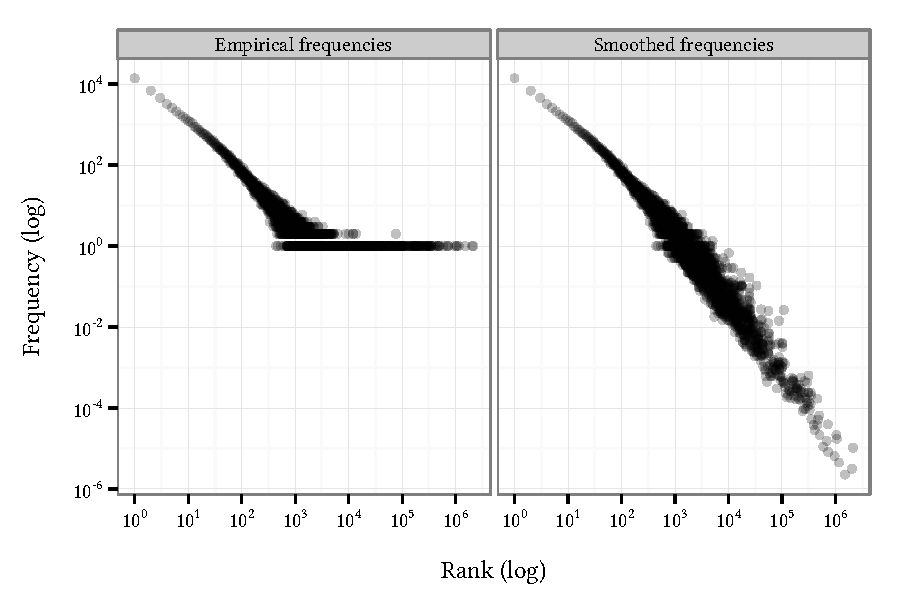
\includegraphics{zr.pdf}
\caption{The left panel shows the empirical word frequencies from the SUBTLEX-US frequency norms \citep{Brysbaert2009}. The right panel shows the same frequencies smoothed with the $Z_r$ transform.}
\label{subtlex}
\end{figure}

\bibliography{gorman_diss.bib}
\bibliographystyle{pwpl}
\end{document}
